\documentclass[12pt]{article}
\usepackage{geometry}
\geometry{a4paper, portrait, margin=1in}

% --- Math Packages ---
\usepackage{amsmath}
\usepackage{amssymb}
\usepackage{amsfonts}
\usepackage{amsthm}

% --- Graphics & Diagrams ---
\usepackage{graphicx}
\usepackage{tikz}
\usetikzlibrary{shapes, arrows, positioning}

% --- Formatting ---
\usepackage{parskip}
\usepackage[hidelinks]{hyperref}
\usepackage{natbib}
\usepackage{enumitem}
\usepackage{booktabs}
\usepackage{caption}
\usepackage{float}
\usepackage{siunitx}
\usepackage{tabularray}
\UseTblrLibrary{booktabs, siunitx}
\pagestyle{plain}

% --- Allow talltblr to break across pages ---
\renewenvironment{table}[1][]{}{}

% --- Word count (requires compiling with --shell-escape) ---
\newcommand{\wordcount}{%
  \immediate\write18{texcount -sum -1 \jobname.tex 2>/dev/null | python3 -c "import sys; n=sys.stdin.read().strip(); print(f'{int(n):,}') if n.isdigit() else print('?')" > \jobname.wc}%
  \input{\jobname.wc}%
}

\title{MPhil Thesis: Robustness and Sensitivity Analysis}
\author{Mohammad-Shah Karim}
\date{May 2026}

\begin{document}

\maketitle

\begin{center}
  \small Word count: \wordcount
\end{center}

\tableofcontents

\newpage

% -----------------------------------------------------------------------
\section{Robustness and Sensitivity Analysis}
% -----------------------------------------------------------------------

The baseline results are estimated using FEOLS with an ex-ante Medicaid market share measure as a proxy for firm-class exposure to the Medicaid reform. This section examines the sensitivity of these findings to alternative specifications, estimation methods, and treatment of the continuous exposure variable. Each research question is addressed in turn.

% -----------------------------------------------------------------------
\subsection{RQ1: Overall Innovation Response}
% -----------------------------------------------------------------------

\subsubsection{Ex-Post Medicaid Exposure}

The baseline specification uses pre-expansion Medicaid market shares to measure treatment intensity. Ex-post market shares are constructed from realised the Medicaid prescription shares in 2014-2015 as an alternative measure of exposure to the ACA. The window for ex-post shares is restricted to the first two years of the reform in order to capture initial shifts in demand without extending into periods where endogenous response in firm entry or prescribing behaviour, may contaminate the exposure measure. Estimates using ex-post exposure act purely as a robustness check since the measure would still reflect the actual post-expansion demand environment as opposed to being a predetermined exposure measure.

Under the estimated ex-post measure, the patent coefficients are nearly identical to the ex-ante estimates. The pre-expansion coefficients remain small and insignificant, highlighting robustness to the parallel trends assumption while the post-reform coefficients follow the same gradual negative trajectory, growing from $-0.088$ in 2015 to $-0.250$ by 2024 before dropping slightly to $-0.212$ in 2025. These estimates are consistent with the ex-ante result, which also has a 2024 peak at $-0.252$. Similarly, the coefficients for FDA approvals are also in line with the baseline specification, where the coefficients are largely statistically insignificant with the exception of 2017 and 2019, while having no clear directional pattern. The alignment between the ex-ante and ex-post results therefore indicates that the findings are orthogonal to the choice of exposure measure.

\begin{figure}[!h]
  \centering
  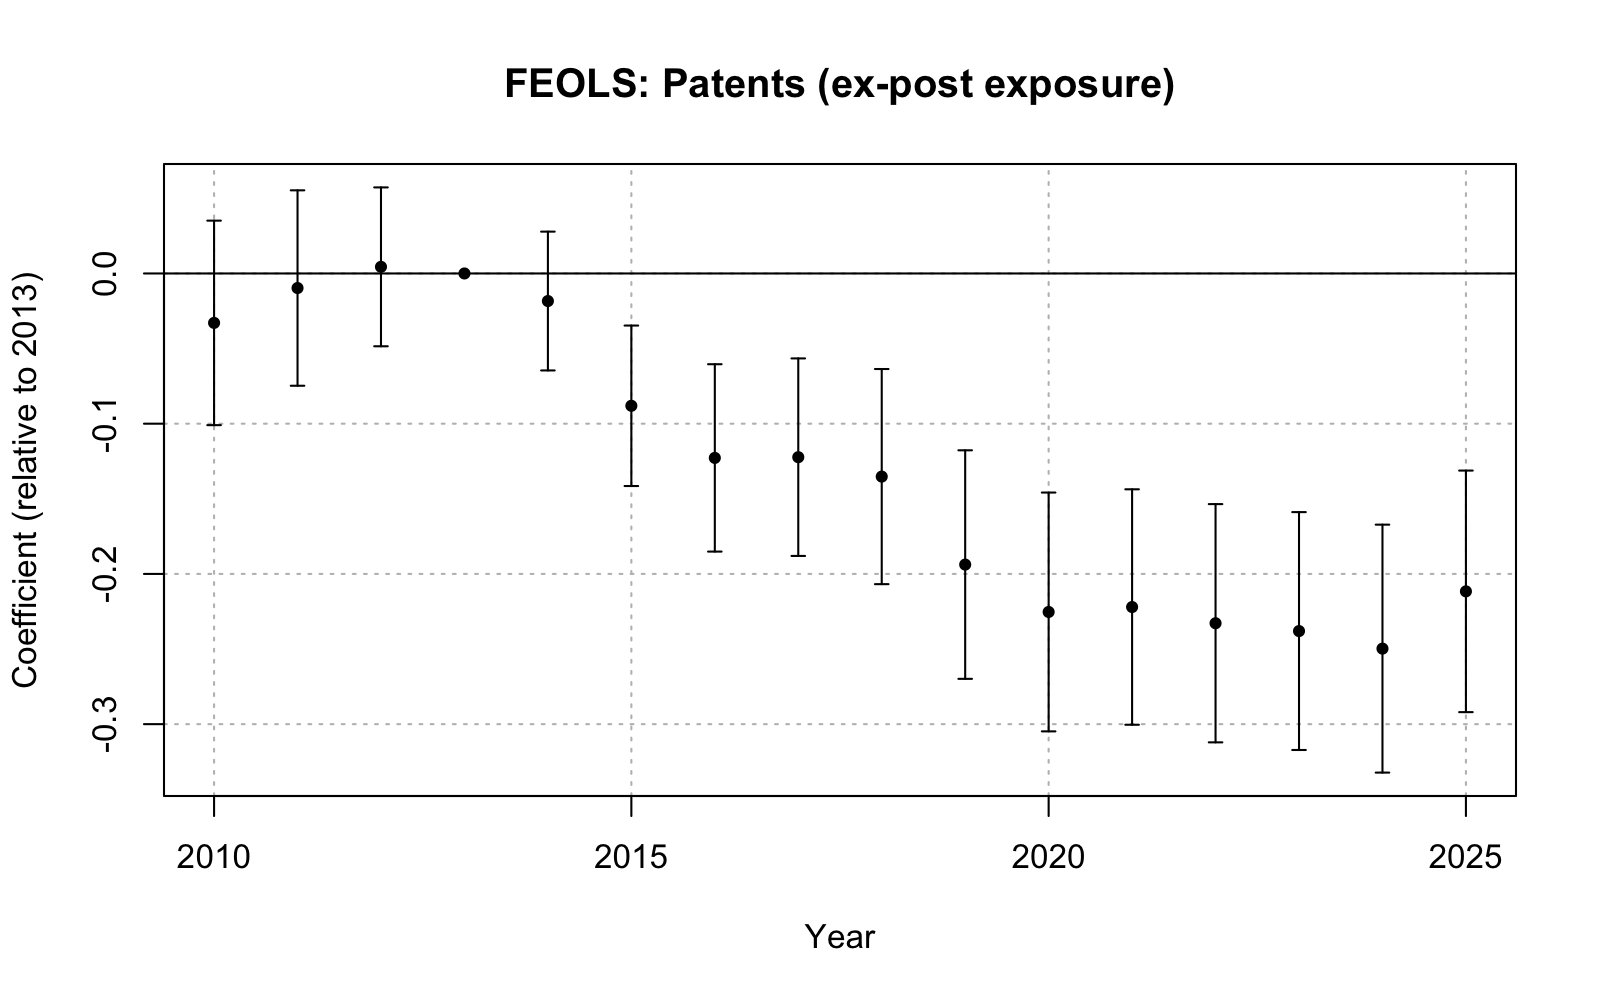
\includegraphics[width=\linewidth]{../output/RQ1/patent_feols_expost.png}
  \caption{FEOLS event study: patents, ex-post Medicaid exposure}
  \label{fig:rob_rq1_patent_feols_expost}
\end{figure}

\begin{figure}[!h]
  \centering
  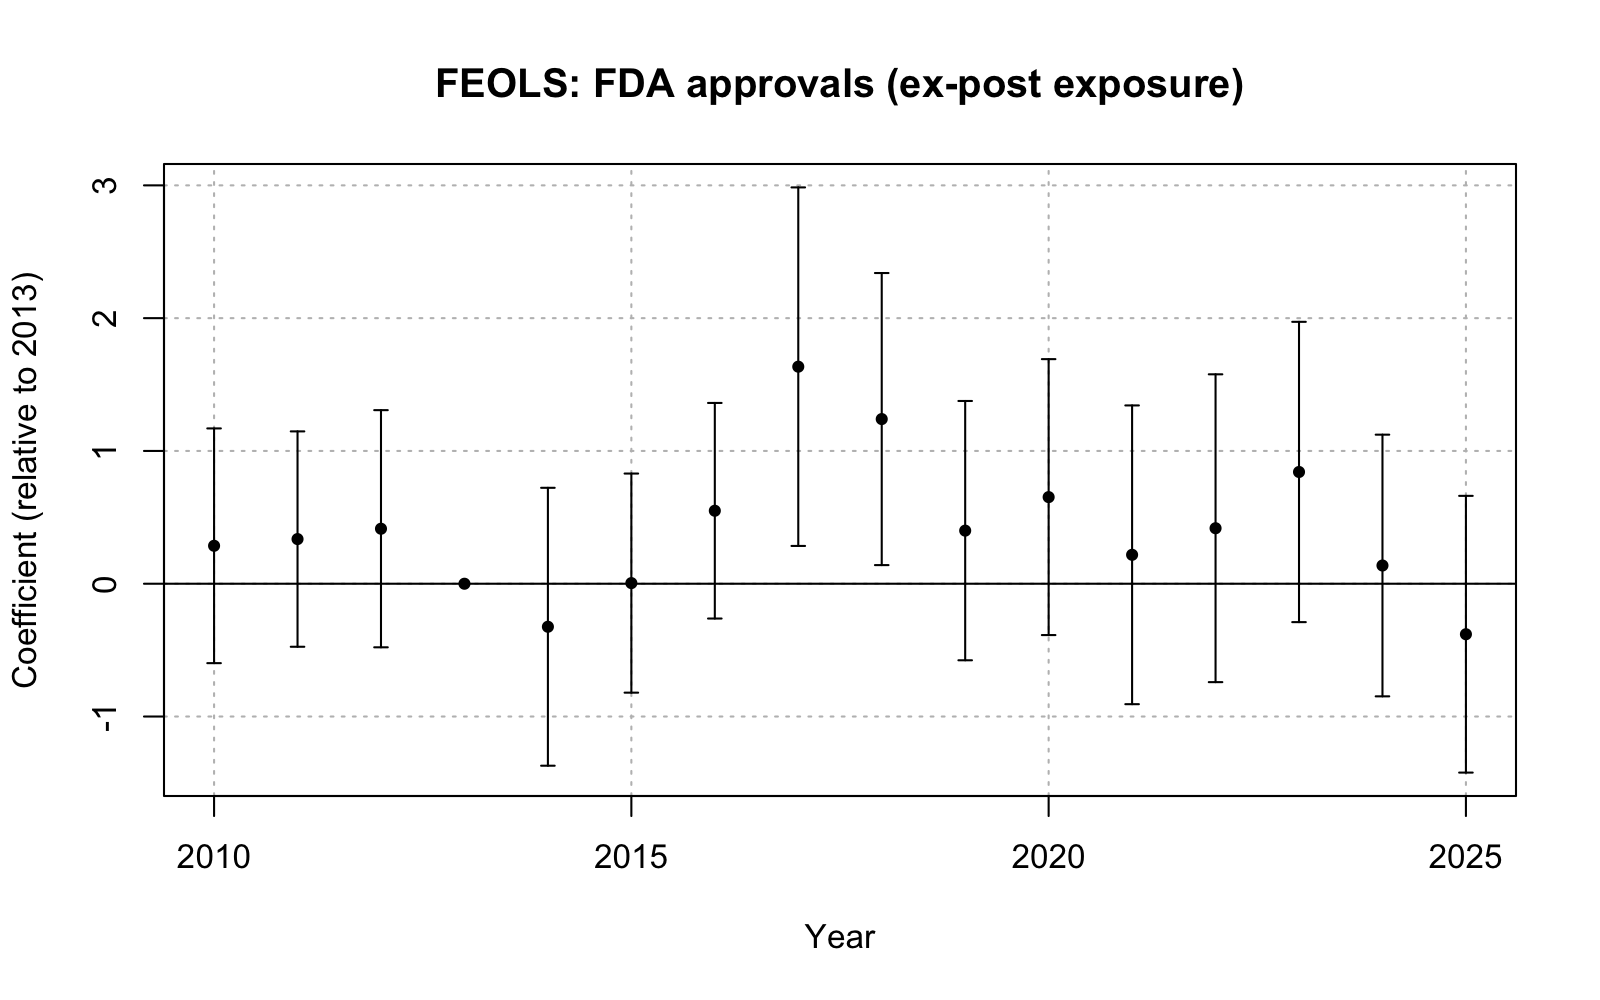
\includegraphics[width=\linewidth]{../output/RQ1/fda_feols_expost.png}
  \caption{FEOLS event study: FDA approvals, ex-post Medicaid exposure}
  \label{fig:rob_rq1_fda_feols_expost}
\end{figure}

\clearpage

\subsubsection{FE Poisson Estimation}

The baseline FEOLS specification models patent counts and FDA approvals linearly, although both outcomes are non-negative integer variables with substantial counts of zero. Consequently, the specification is re-estimated using a fixed-effects Poisson model, which therefore models the conditional mean of each of the innovation outcomes non-linearly. This allows for a robustness check on whether the baseline findings are sensitive to the linear treatment of the count outcomes, since the Poisson estimator remains consistent even when the outcome is overdispersed provided the conditional mean is correctly specified \citep{wooldridge1999distribution}.

The FE Poisson estimates for patents are consistent with the FEOLS results. Under the ex-ante specification, the pre-expansion coefficients are small and insignificant, providing support for the parallel trends assumption. The post-expansion coefficients are negative and grow in magnitude over time, peaking at $-1.474$ by 2024 and fall slightly in 2025, consistent with the FEOLS findings. Therefore, at its peak in 2024, a ten percentage point increase in Medicaid exposure corresponds to an approximate 14.7 percent decrease in patents on average. The ex-post FE Poisson estimates follow a similar trajectory, with the 2024 peak being more negative at $-2.021$.

While the FDA approval estimates under the Poisson model are uniformly negative, they still remain insignificant across both the ex-ante and ex-post specifications. This is a slight deviation from the baseline OLS results, where the FDA estimates fluctuate in sign, but both specifications agree that the innovation response at the approval stage remains statistically significant. The findings for both innovation outcomes are consistent between the linear and Poisson specifications, suggesting that the post-expansion patterns are not sensitive to modelling the count outcomes linearly.

\begin{figure}[!h]
  \centering
  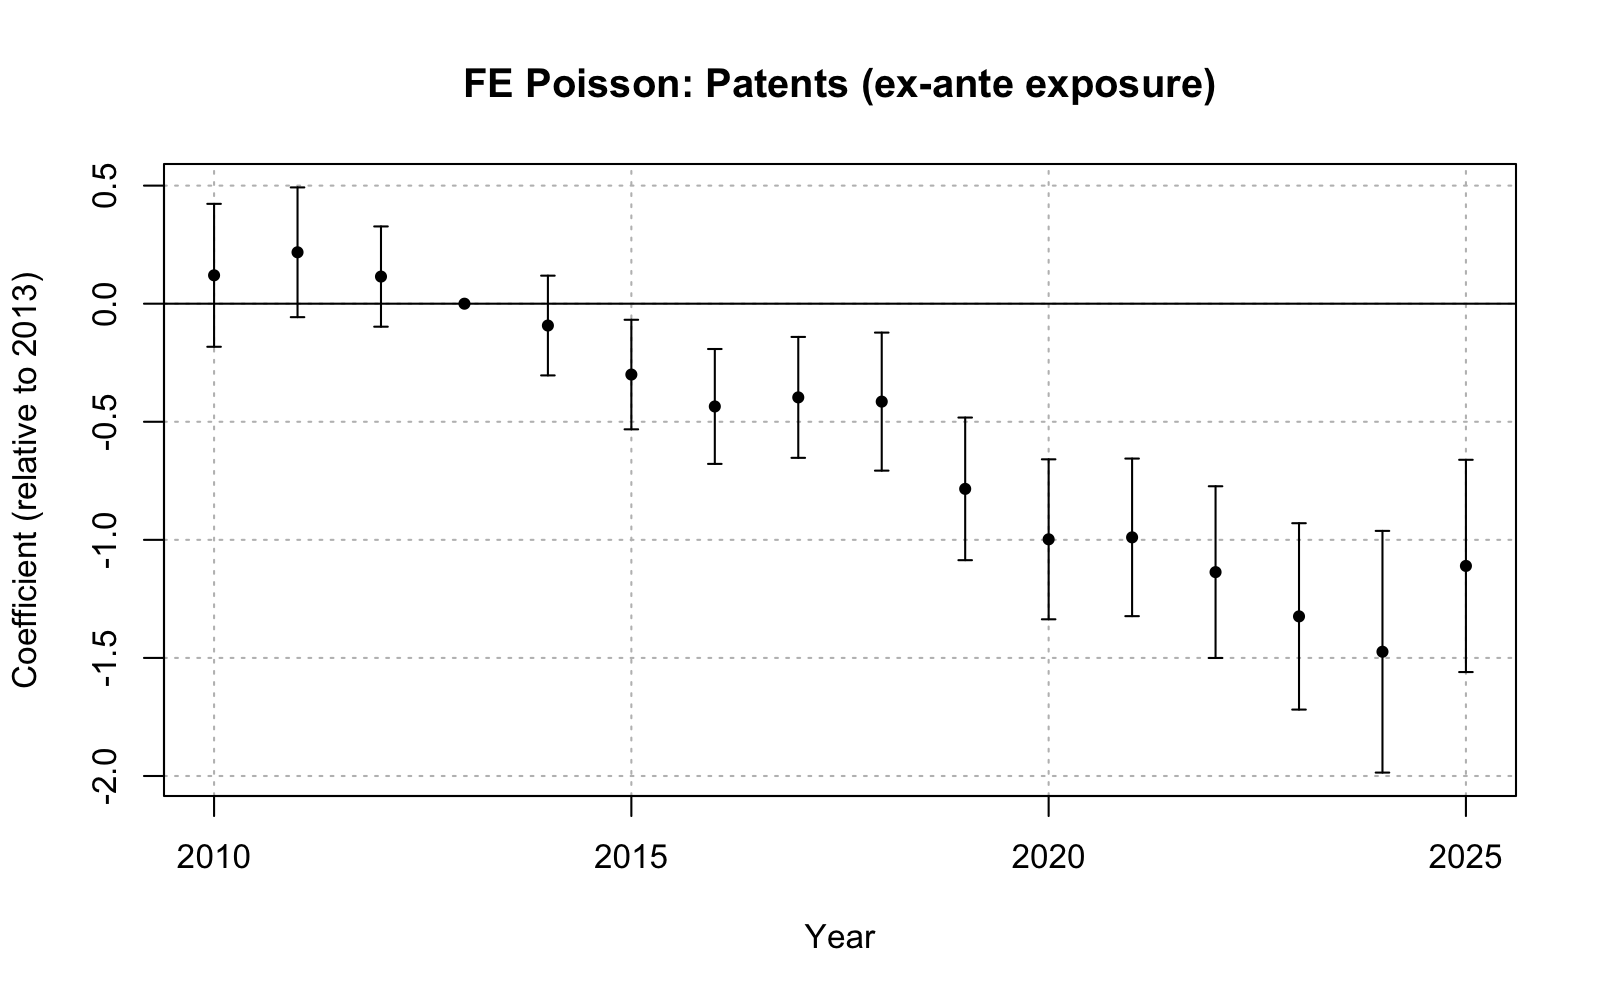
\includegraphics[width=\linewidth]{../output/RQ1/patent_poi_exante.png}
  \caption{FE Poisson event study: patents, ex-ante Medicaid exposure}
  \label{fig:rob_rq1_patent_poi_exante}
\end{figure}

\begin{figure}[!h]
  \centering
  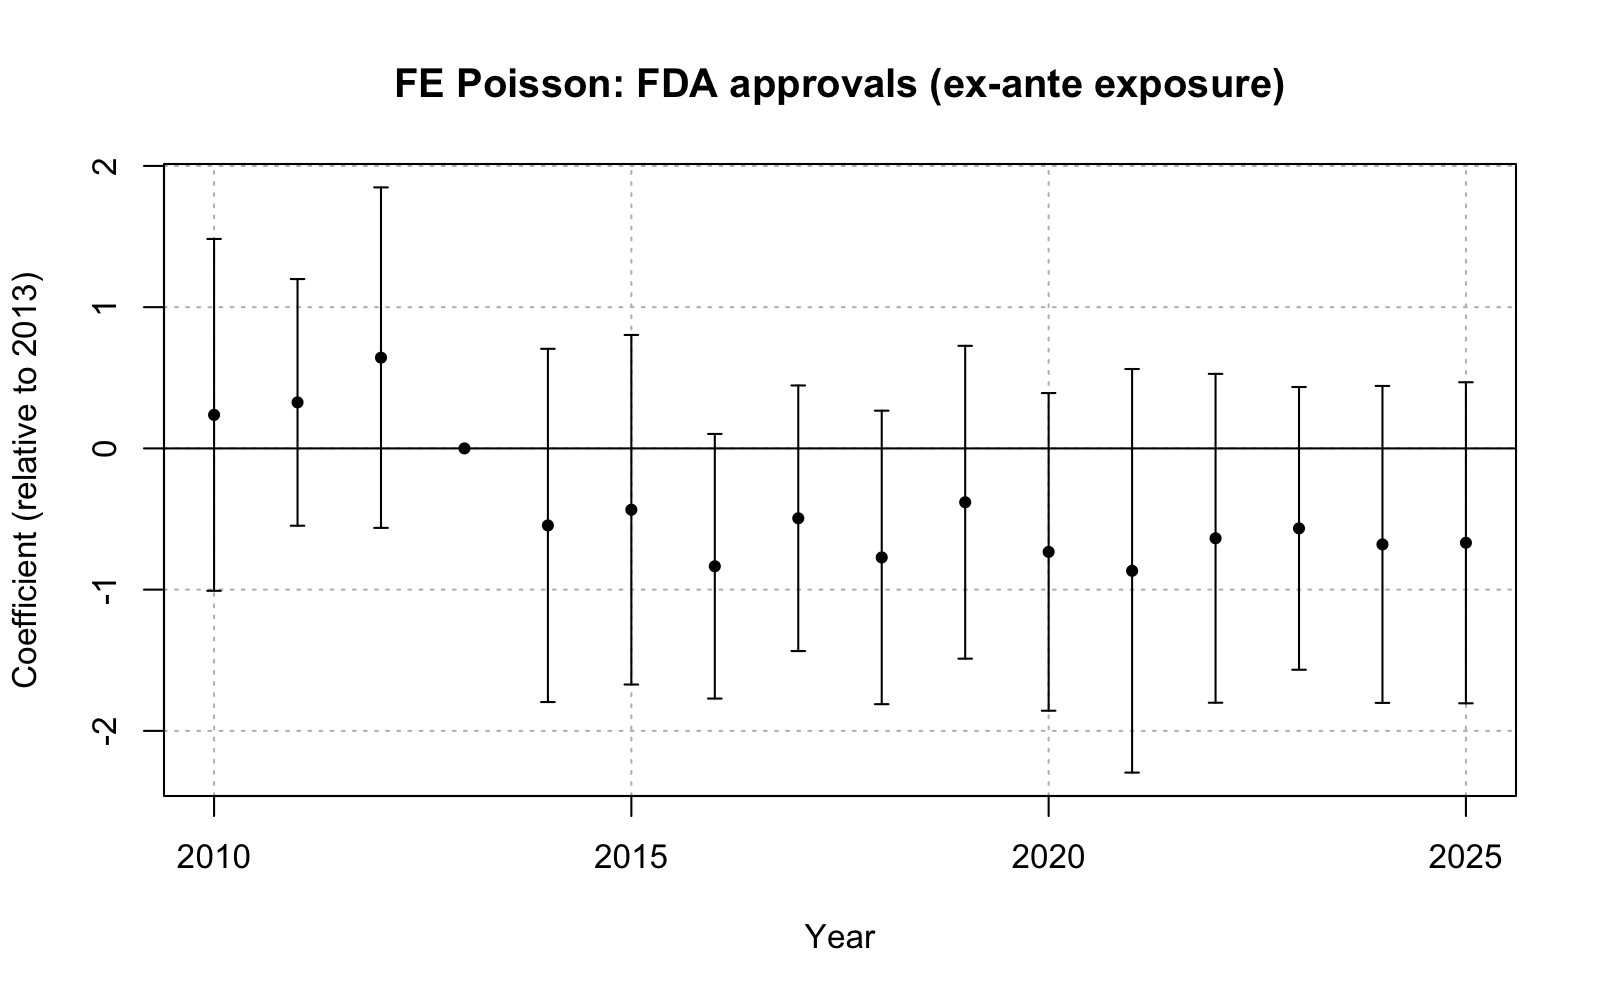
\includegraphics[width=\linewidth]{../output/RQ1/fda_poi_exante.png}
  \caption{FE Poisson event study: FDA approvals, ex-ante Medicaid exposure}
  \label{fig:rob_rq1_fda_poi_exante}
\end{figure}

\clearpage

\subsubsection{Binned Treatment Intensity}

The baseline specification treats exposure to the ACA as a continuous variable. As an alternative test, therapeutic classes are grouped into low, medium and high exposure bins, allowing for separate event-study coefficients to be estimated across different parts of the Medicaid exposure distribution. This relaxes the assumption of linearity in treatment effects imposed by the continuous specification, and examines whether the post-expansion response is concentrated among classes which are greater exposed to the Medicaid reform.

Therapeutic classes are grouped into the three bins based on their ex-ante Medicaid market shares, as reported in Table~\ref{tab:atc_bins}. Nervous system and cardiovascular drugs form the high-exposure bin, as their Medicaid market shares are substantially larger than other class shares. An approximate threshold of 10\% is used to distinguish between the medium and low bin classes, thus anti-infectives and dermatologicals form the medium-exposure bin.


\begingroup
\makeatletter
\renewenvironment{table}[1][tbp]{\@float{table}[#1]}{\end@float}
\makeatother
\begin{table}[htbp]
\centering
\caption{Pre-expansion Medicaid market shares and bin assignments}
\label{tab:atc_bins}
\begin{tabular}{llrl}
\toprule
\multicolumn{1}{c}{ATC} & \multicolumn{1}{c}{Therapeutic Area} & \multicolumn{1}{c}{Medicaid Share} & \multicolumn{1}{c}{Bin} \\
\midrule
N & Nervous system                  & 0.363 & High   \\
C & Cardiovascular system           & 0.215 & High   \\
J & Anti-infectives for systemic use & 0.120 & Medium \\
D & Dermatologicals                 & 0.099 & Medium \\
R & Respiratory system              & 0.085 & Low    \\
A & Alimentary tract and metabolism & 0.068 & Low    \\
M & Musculo-skeletal system         & 0.015 & Low    \\
H & Systemic hormonal preparations  & 0.012 & Low    \\
L & Antineoplastic and immunomodulating agents & 0.006 & Low \\
G & Genito-urinary system and sex hormones     & 0.006 & Low \\
S & Sensory organs                  & 0.005 & Low    \\
B & Blood and blood-forming organs  & 0.005 & Low    \\
V & Various                         & 0.000 & Low    \\
P & Antiparasitic products          & 0.000 & Low    \\
\bottomrule
\end{tabular}
\end{table}

\endgroup

The low exposure bin is omitted from the regression, so the coefficients for the high and medium bins are estimated relative to the low-exposure bin. The pre-expansion coefficients for both the high and medium-exposure patent bins are small and statistically insignificant, supporting the parallel trends assumption within each group. While the medium-exposure bin largely contain positive insignificant coefficients throughout the post-expansion period with a peak decline of $-0.02$ in 2025, the high-exposure bin exhibit a growing negative trajectory with coefficients reaching $-0.155$ by the same year. This reinforces the finding from RQ3 that the post-expansion patenting decline driven by classes at the upper end of the Medicaid exposure distribution. Importantly, the relative magnitude of the high and medium exposure coefficients is disproportionately larger than their respective Medicaid market shares. On average, exposure of the high bin is approximately $2.5$ times larger than the medium bin, yet the peak patent responses approximately differ by a factor of eight. This suggests that the relationship between Medicaid exposure and patenting may be convex, with the response intensifying at greater levels of exposure as opposed to scaling proportionally.

FDA approval estimates are statistically insignificant for both the high and medium-exposure bins throughout the sample period, and the pre-expansion coefficients are close to zero in both bins, supporting the parallel trends assumption. The absence of significant post-expansion effects for FDA approvals is consistent with the baseline findings and reinforces the interpretation that the innovation response has not yet propagated to the downstream approval stage. Unlike the patent results, the estimates from the FDA binned specification provide no evidence of a non-linear treatment effects across the Medicaid market share distribution, but this is driven by the absence of a detectable effect within each of the exposure bins rather than providing support for a linear relationship.

\clearpage

\begin{figure}[!h]
  \centering
  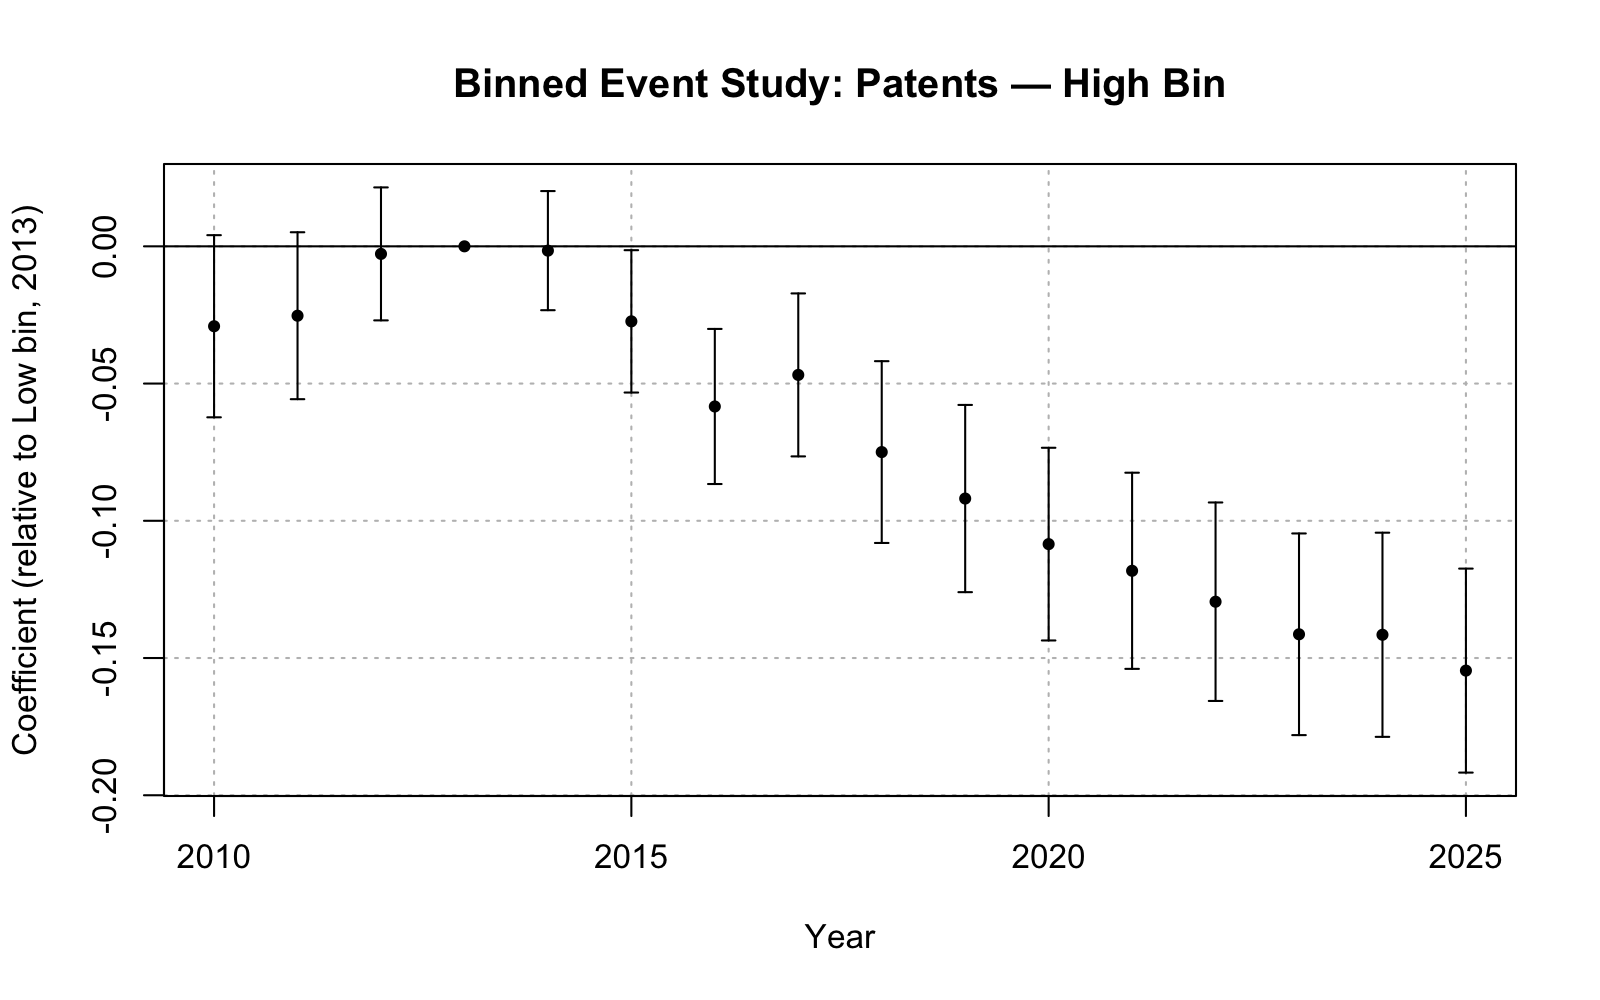
\includegraphics[width=\linewidth]{../output/robustness/binned_treatment/binned_patent_high_es.png}
  \caption{Binned event study: patents, high-exposure bin (N, C)}
  \label{fig:rob_binned_patent_high}
\end{figure}

\begin{figure}[!h]
  \centering
  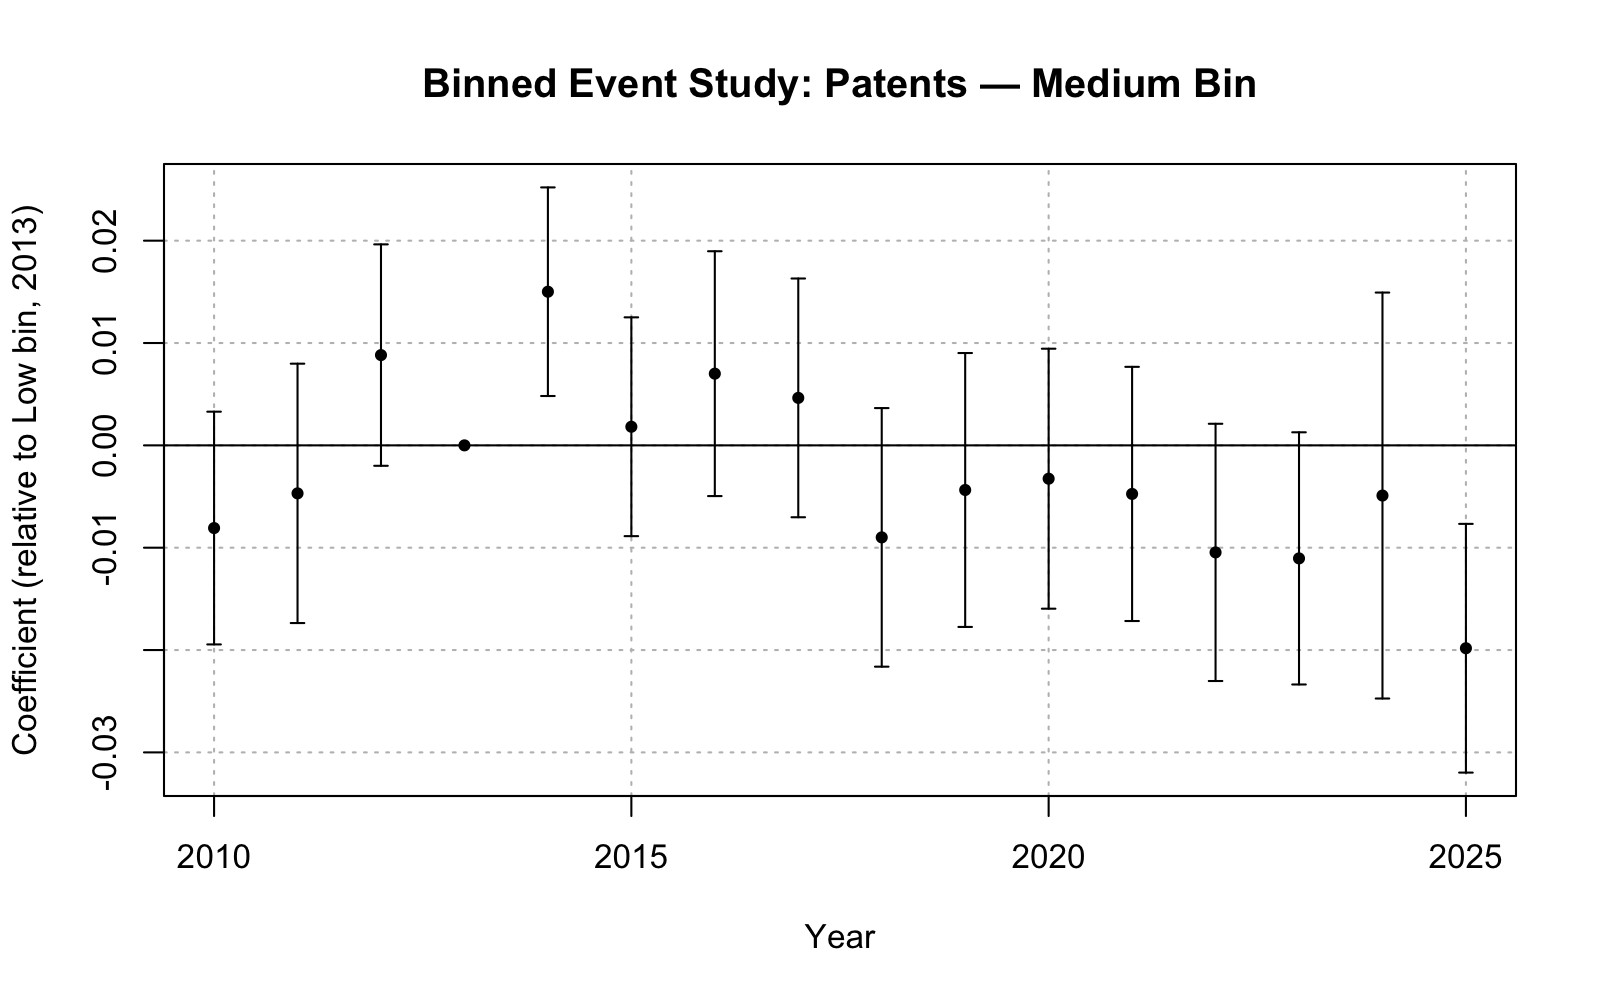
\includegraphics[width=\linewidth]{../output/robustness/binned_treatment/binned_patent_medium_es.png}
  \caption{Binned event study: patents, medium-exposure bin (J, D)}
  \label{fig:rob_binned_patent_medium}
\end{figure}

\clearpage

\begin{figure}[!h]
  \centering
  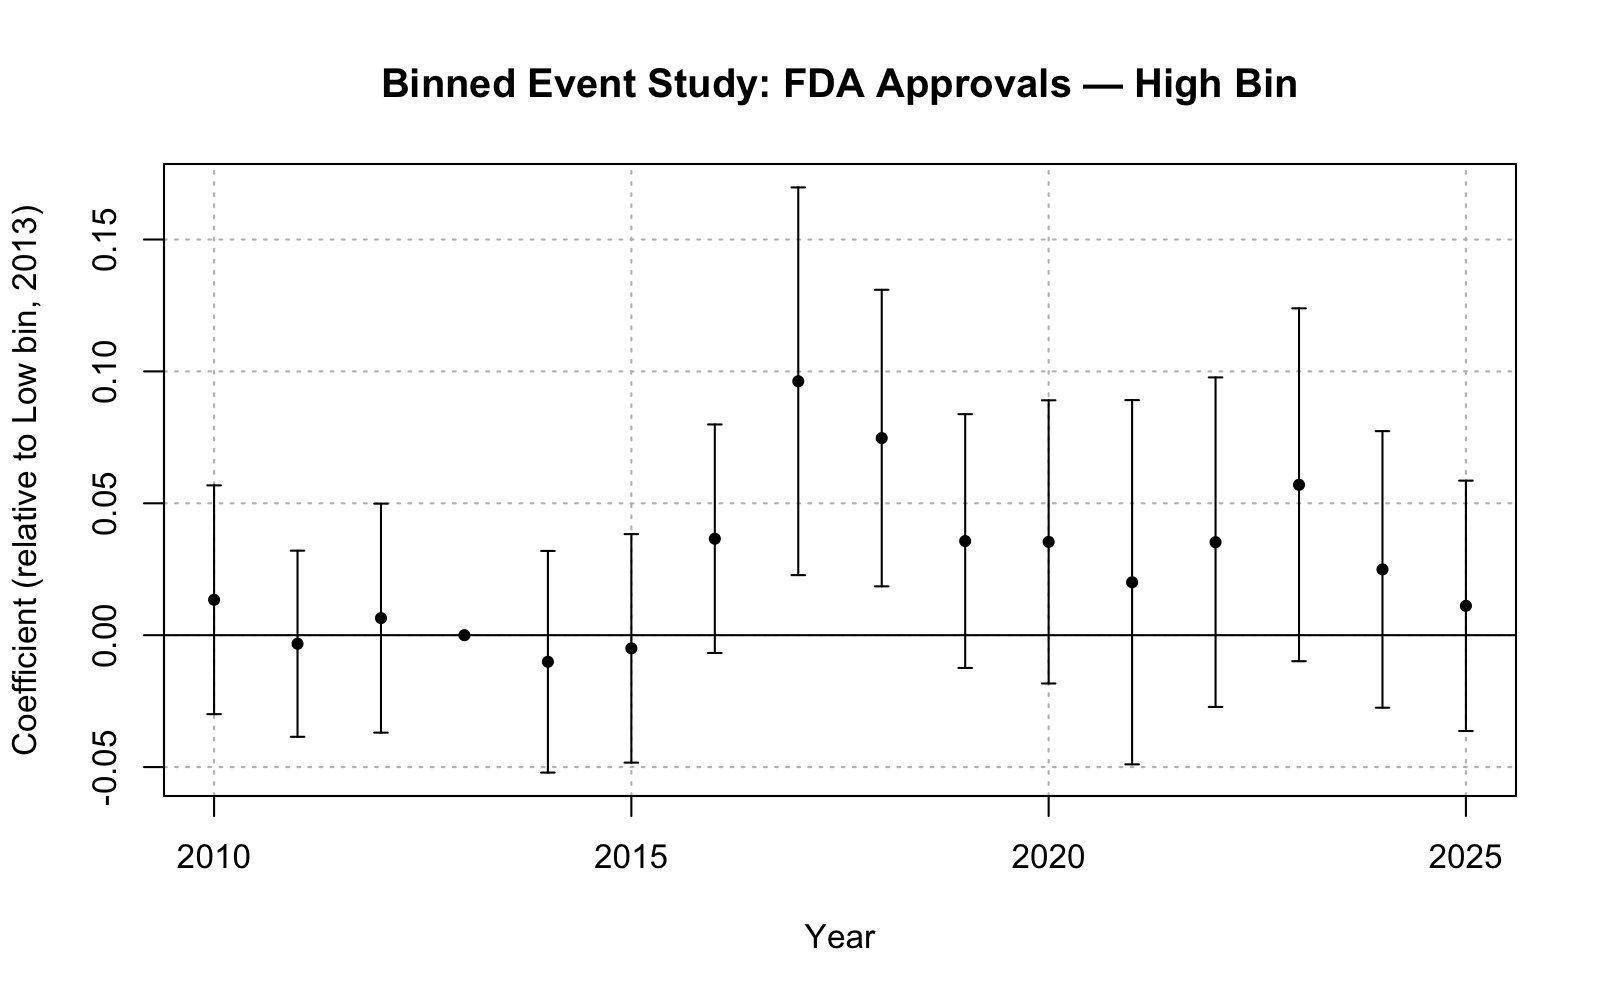
\includegraphics[width=\linewidth]{../output/robustness/binned_treatment/binned_fda_high_es.png}
  \caption{Binned event study: FDA approvals, high-exposure bin (N, C)}
  \label{fig:rob_binned_fda_high}
\end{figure}

\begin{figure}[!h]
  \centering
  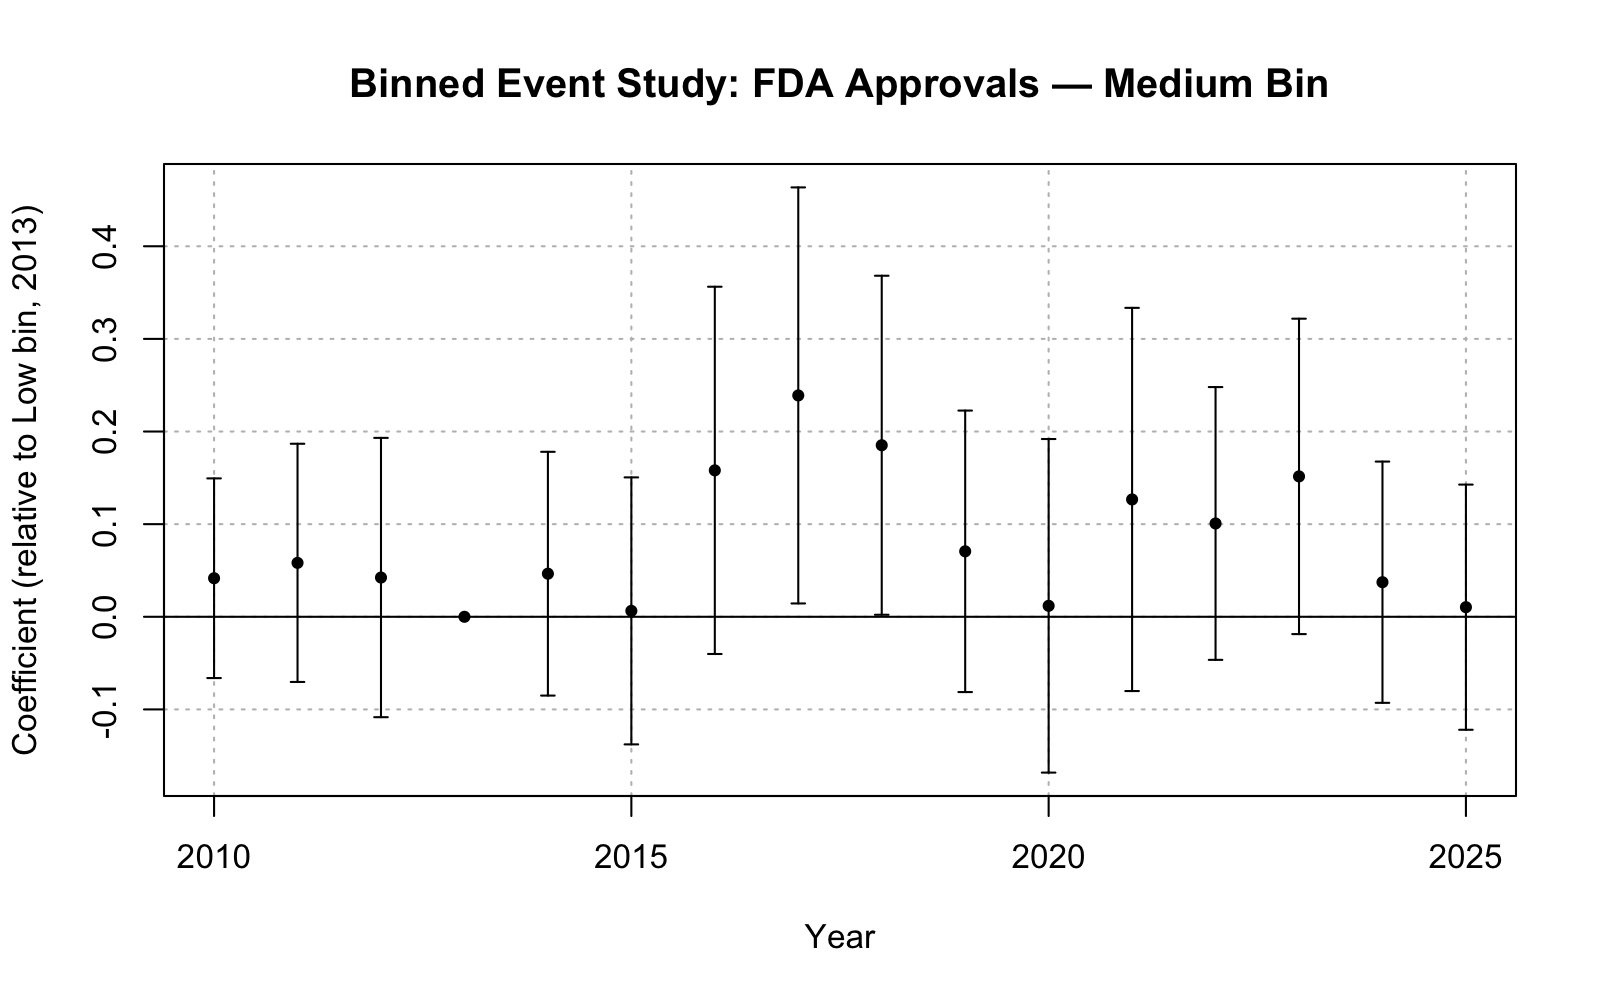
\includegraphics[width=\linewidth]{../output/robustness/binned_treatment/binned_fda_medium_es.png}
  \caption{Binned event study: FDA approvals, medium-exposure bin (J, D)}
  \label{fig:rob_binned_fda_medium}
\end{figure}

\clearpage

\subsubsection{Continuous Difference-in-Differences}

The binned event-study specification allowed for treatment effects to vary across the discrete groups, but the results were contingent on the boundaries specified for each exposure bin. Given this, the continuous difference-in-differences (Continuous DiD) estimator proposed by \citet{NBERw32117} is applied using the \texttt{contdid} R package \citep{contdid2025}. This estimator non-parametrically identifies dose-specific treatment effects at each exposure-level under the parallel trends assumption, thereby avoiding the need to discretise the treatment variable. Conventional TWFE estimators with continuous treatment can be difficult to interpret when treatment effects differ across the distribution of exposure level. The Continuous DiD estimator avoids this by aggregating the dose-specific estimates into event-study coefficients and assesses for pre-trends and post-treatment dynamics. The full set of coefficient estimates is reported in Table~\ref{tab:contdid_es}.

The Continuous DiD estimates for patents are consistent with the baseline results. The pre-expansion coefficients are small and statistically insignificant, supporting the parallel trends assumption. Notably, the coefficients are persistently significant from 2019 onwards, which is four years later than the 2015 onset under the baseline FEOLS model. This implies that the innovation response was not immediate as suggested by the baseline results, instead firms required several years to fully adjust their R\&D decisions in response to the expansion.

The FDA approval estimates under the Continuous DiD model are statistically insignificant throughout the entire period. The pre-period estimates are small and fluctuate around zero, while the post-expansion estimates are mostly positive. The absence of a clear FDA approval response to the Medicaid reform is therefore robust to modelling Medicaid exposure non-parametrically within the Continuous DiD framework.

Taken together, the results from the sensitivity analysis show that the main findings are robust to discretising market shares into exposure bins and using a non-parametric continuous DiD approach. Crucially, the sustained negative patent response remains visible under an estimator developed specifically for continuous-treatment DiD designs, while drug approvals do not appear to have a clear response to the ACA. The Continuous DiD estimates are also consistent with the binned analysis for highly exposed patents, while bins with medium exposure do not display a statistically significant response. This pattern is consistent with the class-level heterogeneity identified in RQ3, where nervous system and cardiovascular drugs were among the classes experiencing the greatest patent reductions.

\clearpage

\begin{figure}[!h]
  \centering
  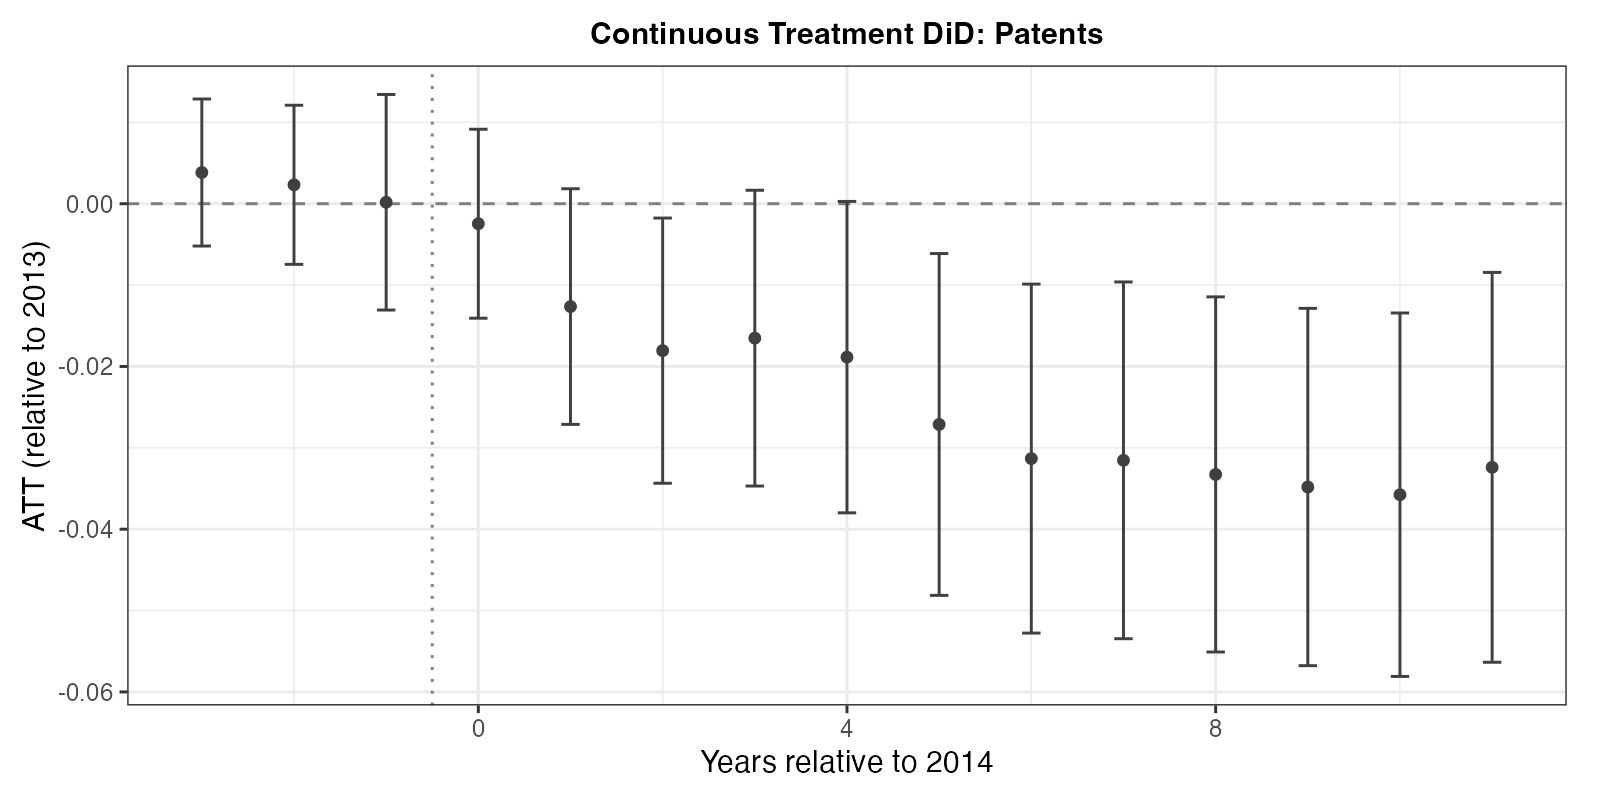
\includegraphics[width=\linewidth]{../output/robustness/contdid/contdid_patent_es.png}
  \caption{Continuous DiD event study: patents}
  \label{fig:rob_contdid_patent}
\end{figure}

\begin{figure}[!h]
  \centering
  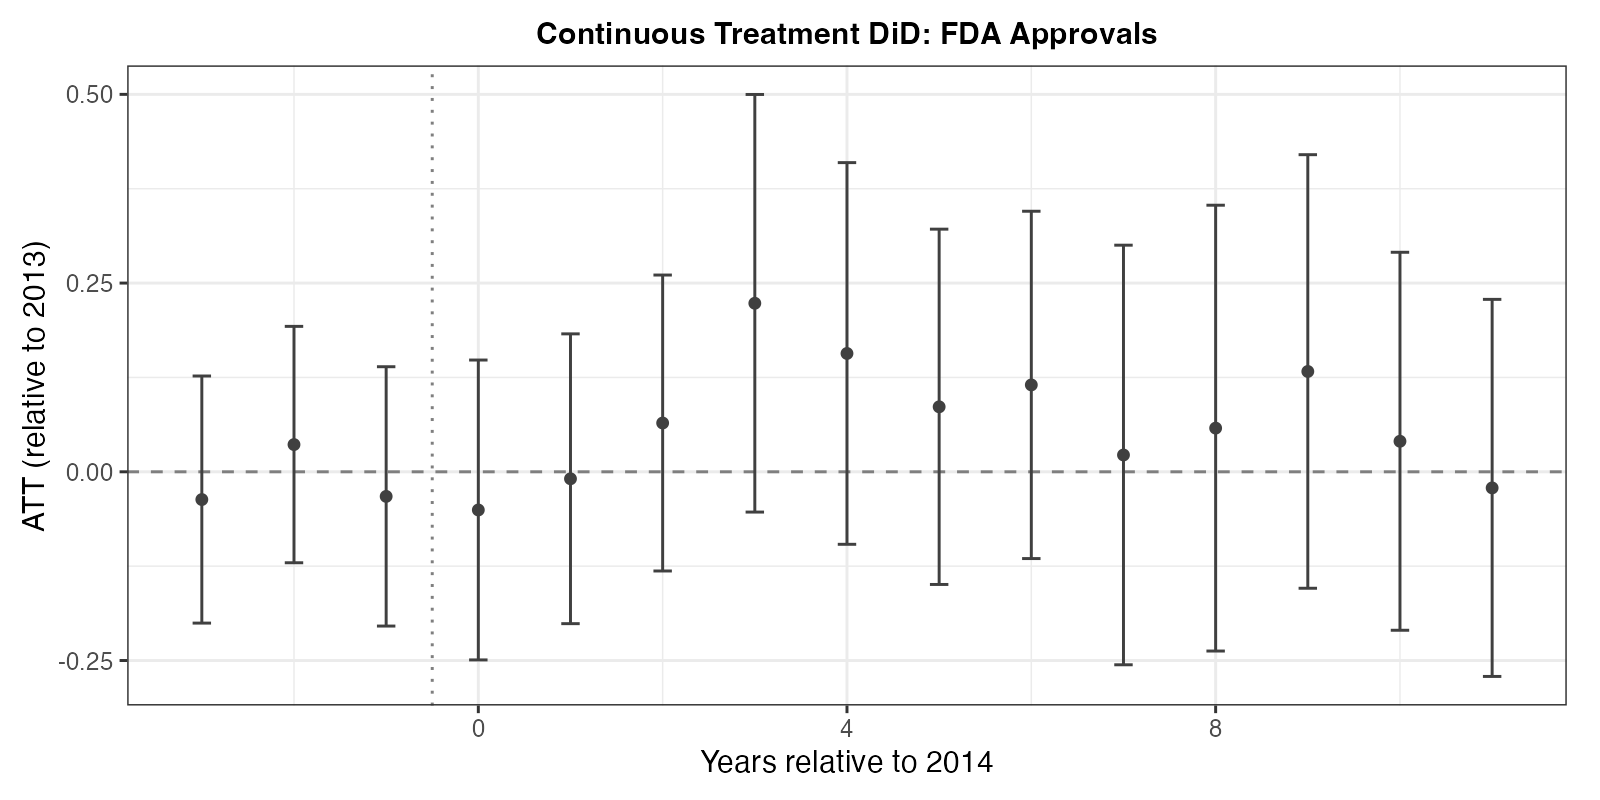
\includegraphics[width=\linewidth]{../output/robustness/contdid/contdid_fda_es.png}
  \caption{Continuous DiD event study: FDA approvals}
  \label{fig:rob_contdid_fda}
\end{figure}

\clearpage

% -----------------------------------------------------------------------
\subsection{RQ2: Medicaid Demand and PDL Exposure}
% -----------------------------------------------------------------------

\subsubsection{Ex-Post Medicaid Exposure}

The second specification jointly estimates the innovation response to Medicaid demand exposure and exposure to the PDL. Like RQ1, an ex-post market share measure is used to determine whether the estimates are sensitive to the construction of the exposure variable.

Once again, the ex-post Medicaid exposure coefficients for patents are nearly identical to the baseline results. The same reductions in Medicaid market share coefficients is observed, with the PDL exposure coefficient path also coinciding with the ex-ante model which saw negative coefficients from 2016 with significance from 2019. The pre-expansion coefficients for both the Medicaid and PDL measures remain small and statistically insignificant, supporting the parallel trends assumption even under the ex-post exposure construction.

The FDA approval coefficients are largely under the ex-post specification are statistically insignificant for both the Medicaid and PDL exposure measures, with isolated incidences of significance in a small number of post-expansion years. This aligns with the baseline finding that the innovation response has not yet reached the final stage of the R\&D pipeline. The agreement between the ex-ante and ex-post results therefore indicates that the decomposition into Medicaid demand and PDL exposure is not sensitive to the construction of exposure to Medicaid.

The FE Poisson, binned treatment, and continuous difference-in-differences estimators are not applied to the RQ2 specification. The joint estimation of two exposure variables under these alternative specifications is computationally demanding, and could not be completed with the device used for this study. Given this constraint, the alternative estimators are only used for the RQ1 specification where they are most informative for the aggregate response to the policy.

\clearpage

\begin{figure}[!h]
  \centering
  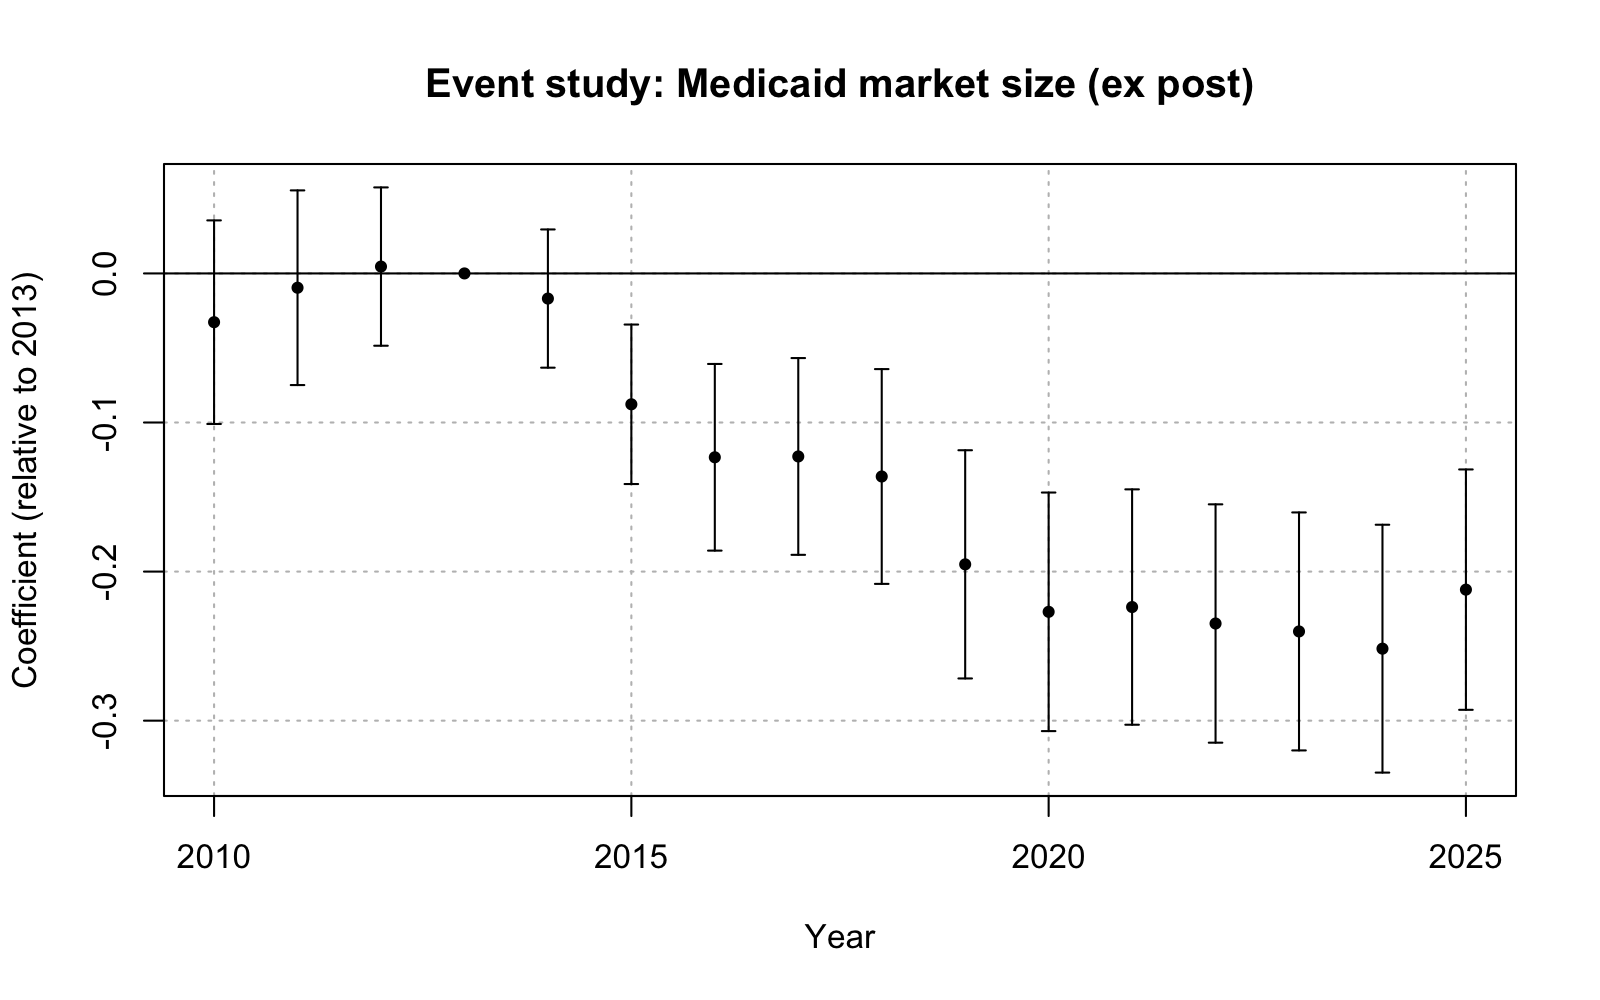
\includegraphics[width=\linewidth]{../output/RQ2/patent_feols_expost_medicaid.png}
  \caption{FEOLS event study: patents, Medicaid exposure (ex-post)}
  \label{fig:rob_rq2_patent_expost_medicaid}
\end{figure}

\begin{figure}[!h]
  \centering
  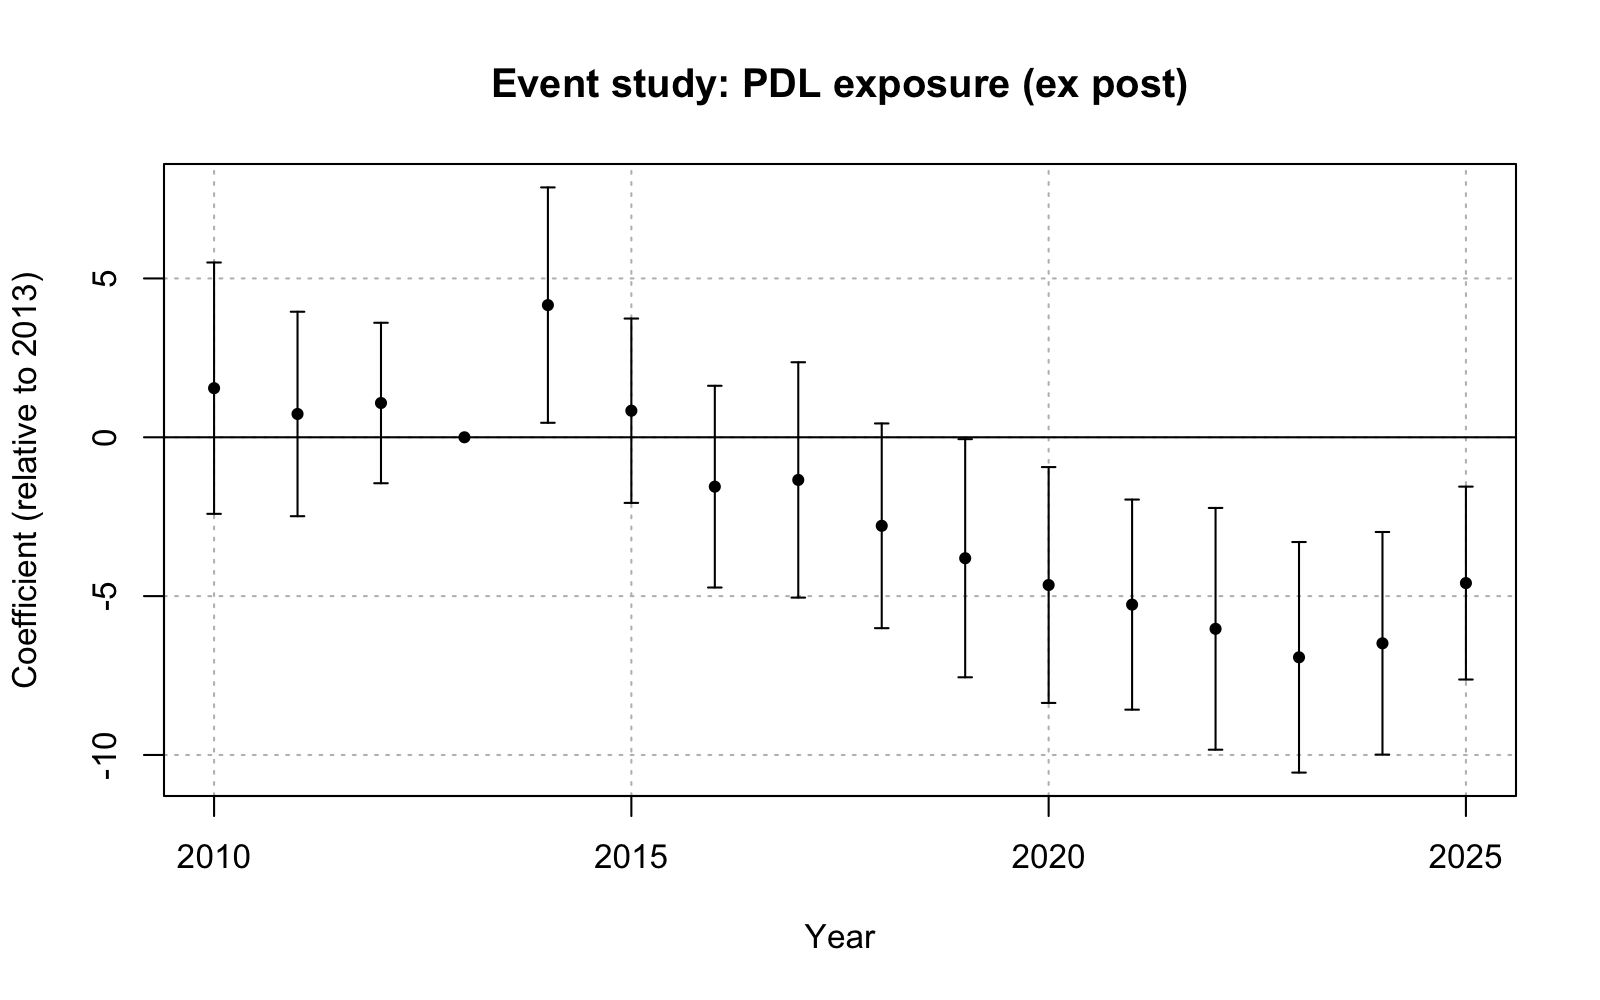
\includegraphics[width=\linewidth]{../output/RQ2/patent_feols_expost_pdl.png}
  \caption{FEOLS event study: patents, PDL exposure (ex-post)}
  \label{fig:rob_rq2_patent_expost_pdl}
\end{figure}

\clearpage

\begin{figure}[!h]
  \centering
  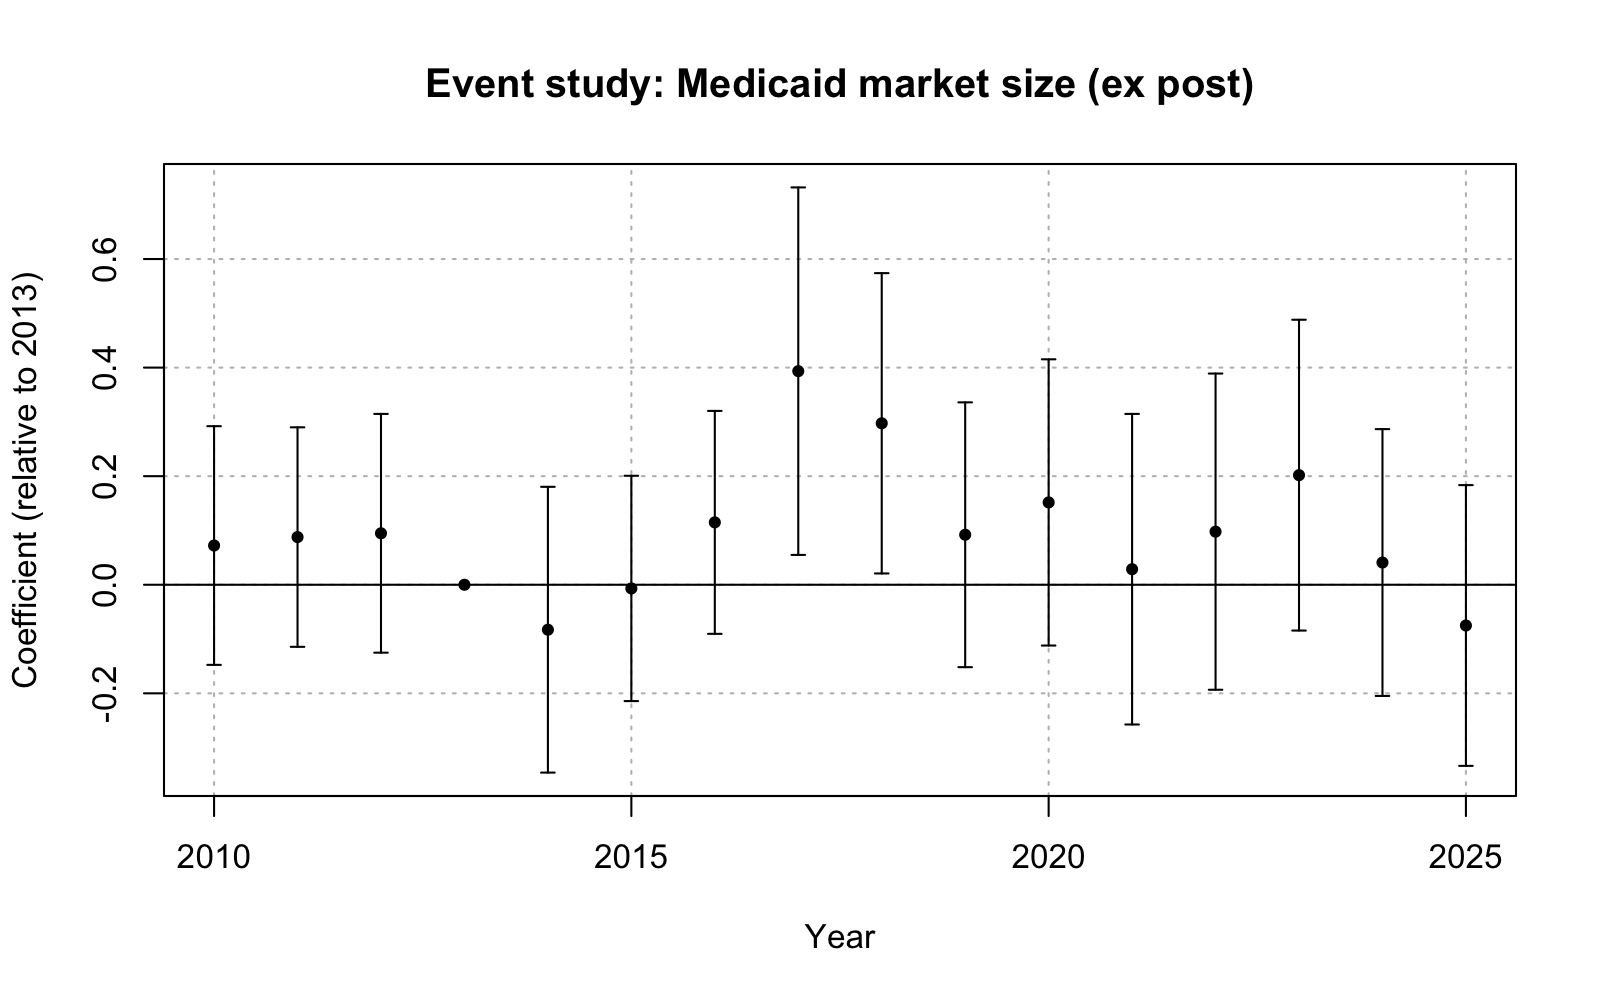
\includegraphics[width=\linewidth]{../output/RQ2/fda_feols_expost_medicaid.png}
  \caption{FEOLS event study: FDA approvals, Medicaid exposure (ex-post)}
  \label{fig:rob_rq2_fda_expost_medicaid}
\end{figure}

\begin{figure}[!h]
  \centering
  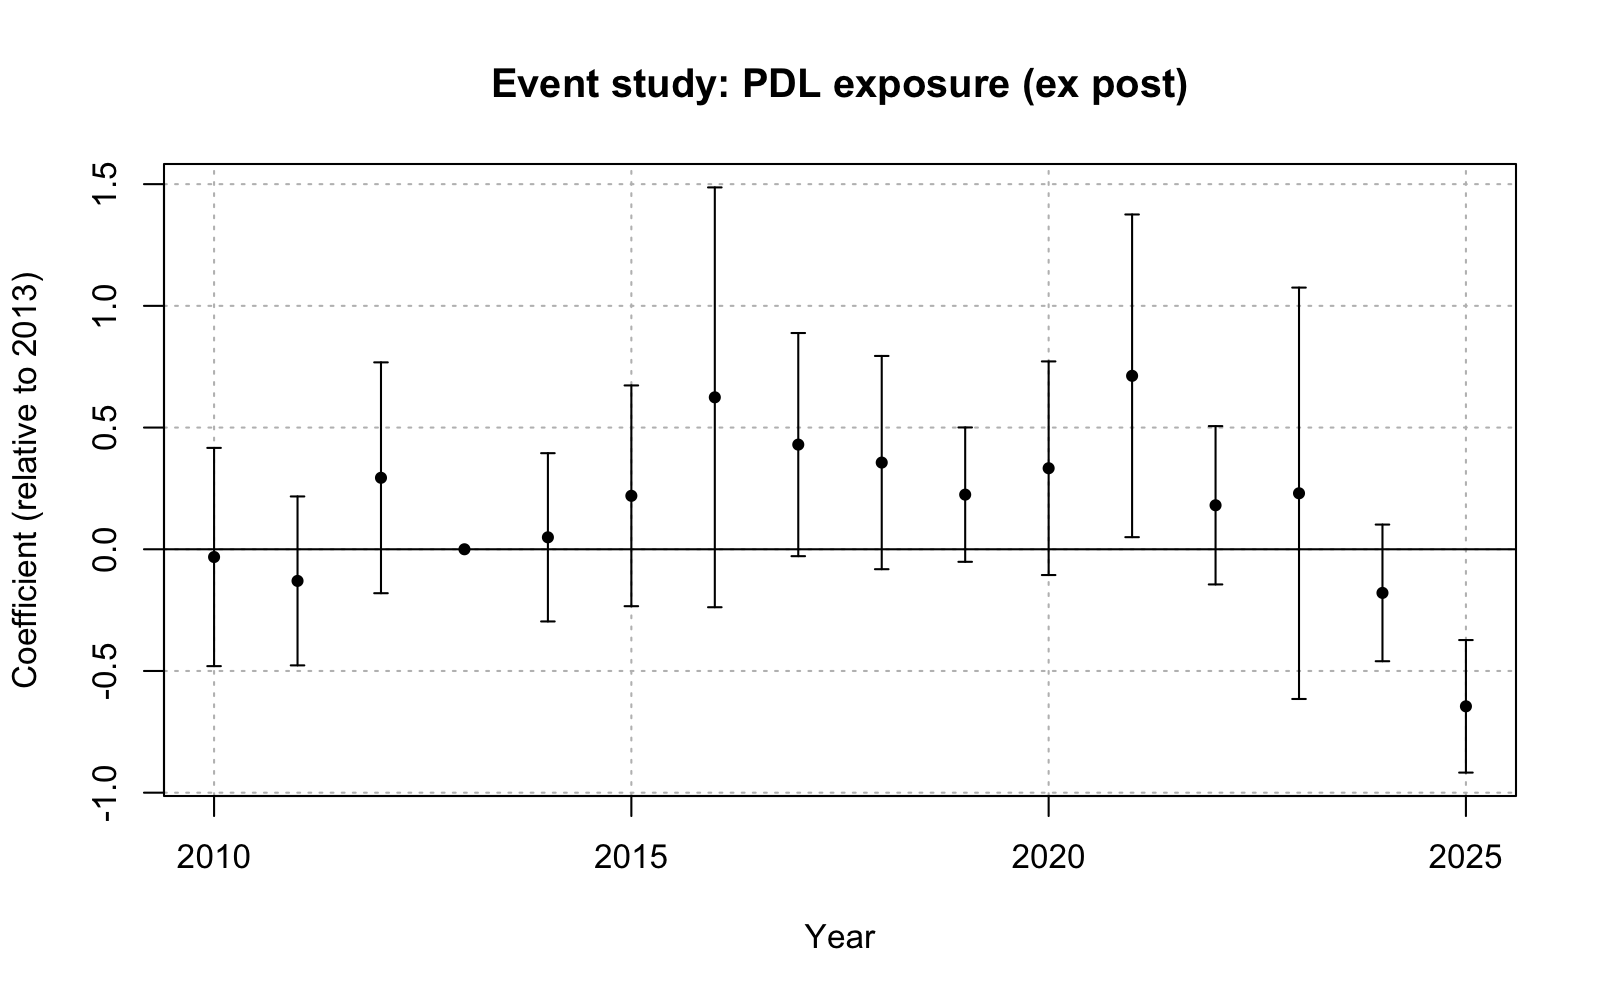
\includegraphics[width=\linewidth]{../output/RQ2/fda_feols_expost_pdl.png}
  \caption{FEOLS event study: FDA approvals, PDL exposure (ex-post)}
  \label{fig:rob_rq2_fda_expost_pdl}
\end{figure}

\clearpage

% -----------------------------------------------------------------------
\subsection{RQ3: Therapeutic-Class Heterogeneity}
% -----------------------------------------------------------------------

\subsubsection{Ex-Post Medicaid Exposure}

The RQ3 specification allows for heterogeneity in innovation behaviour to vary at ATC Level 1 therapeutic class. The ex-post exposure measure of Medicaid exposure is used as a robustness check.

\begin{center}
\begingroup\footnotesize
\begin{table}
\centering
\begin{talltblr}[         %% tabularray outer open
entry=none,label=none,
note{}={* p \num{< 0.05}, ** p \num{< 0.01}, *** p \num{< 0.001}},
]                     %% tabularray outer close
{                     %% tabularray inner open
colspec={Q[]Q[]Q[]},
column{2,3}={}{halign=c,},
column{1}={}{halign=l,},
hline{26}={1,2,3}{solid, black, 0.05em},
}                     %% tabularray inner close
\toprule
& Patents & FDA Approvals \\ \midrule
Medicaid Share × ATC = A & \num{-0.157}*** & \num{1.301}**  \\
& (\num{0.031})   & (\num{0.420})  \\
Medicaid Share × ATC = B & \num{0.151}***  & \num{-0.121}   \\
& (\num{0.027})   & (\num{0.784})  \\
Medicaid Share × ATC = C & \num{-0.094}*** & \num{0.373}    \\
& (\num{0.015})   & (\num{0.278})  \\
Medicaid Share × ATC = D & \num{-0.017}    & \num{0.881}**  \\
& (\num{0.062})   & (\num{0.337})  \\
Medicaid Share × ATC = G & \num{0.032}     & \num{-1.058}   \\
& (\num{0.049})   & (\num{1.121})  \\
Medicaid Share × ATC = H & \num{0.619}***  & \num{0.446}    \\
& (\num{0.096})   & (\num{0.530})  \\
Medicaid Share × ATC = J & \num{0.035}     & \num{-0.078}   \\
& (\num{0.034})   & (\num{0.089})  \\
Medicaid Share × ATC = L & \num{0.443}     & \num{-0.244}   \\
& (\num{0.578})   & (\num{2.115})  \\
Medicaid Share × ATC = M & \num{-0.212}*** & \num{0.017}    \\
& (\num{0.048})   & (\num{0.858})  \\
Medicaid Share × ATC = N & \num{-0.174}*** & \num{0.047}    \\
& (\num{0.039})   & (\num{0.101})  \\
Medicaid Share × ATC = R & \num{0.005}     & \num{0.178}    \\
& (\num{0.003})   & (\num{0.130})  \\
Medicaid Share × ATC = S & \num{0.105}***  & \num{6.473}*   \\
& (\num{0.020})   & (\num{3.004})  \\
Num. obs.                & \num{19617728}  & \num{561600}   \\
R2                       & \num{0.247}     & \num{0.235}    \\
\bottomrule
\end{talltblr}
\end{table}

\endgroup
\end{center}


The ex-post estimates are broadly consistent with the ex-ante baseline. Therapeutic classes that exhibited significant negative patent responses under ex-ante exposure, continue to display significant negative coefficients under the ex-post measure. Additionally, positive patent responses are still observed for therapeutic classes relating to blood related drugs, hormonal preparations, and sensory organs. Simiarly, the FDA approval coefficients are aligned with their ex-ante results - significant positive responses for alimentary tract and dermatologicals, and no class are recorded to have a significant reduction in approvals. The results aligning between the two exposure measures indicates that the baseline class-level heterogeneity in innovation response is not driven by the choice of exposure measure.

\subsubsection{Parallel Trends}

The RQ3 triple-difference specification does not take the form of an event study, as the estimation of class-specific dynamic coefficients would be computationally intensive. Consequently, pre-trends coefficients cannot be estimated directly, so the parallel trends assumption cannot be tested for in the same manner as RQ1 and RQ2. Since ATC class V is the omitted from the regressions, it is the reference group for the DDD models. In this context, this specifically indicates that absent the ACA, the relationship between Medicaid exposure and changes in innovation outcomes would have evolved similarly across therapeutic classes relative to class V. The results from earlier the earlier analyses and the model structure can provide evidence to support the plausibility of this assumption.

First, the RQ1 and RQ2 event studies consistently display small and statistically insignificant pre-expansion coefficients across all specifications, including FEOLS, FE Poisson, binned treatment and the continuous DiD approach. Therefore, therapeutic classes with differing levels of Medicaid exposure followed similar innovation trajectories prior to the ACA expansion. Since the same Medicaid exposure measure and firm-class panels are used for RQ3, the evidence for parallel trends from RQ1 and RQ2 provide support for the key identifying assumption of RQ3.

Third, as discussed in the methodology, a violation of parallel trends would require an additional shock around 2014 that differentially affected innovation within therapeutic classes such that it was correlated with exposure to Medicaid. There are no clear candidates for such a confounding shock.

\clearpage

\bibliographystyle{apalike}
\bibliography{references}

\clearpage
\appendix

% -----------------------------------------------------------------------
\section{Robustness Regression Tables}
% -----------------------------------------------------------------------

\subsection{RQ1: Ex-Post FEOLS}

\begingroup\footnotesize
\begin{table}
\centering
\begin{talltblr}[         %% tabularray outer open
entry=none,label=none,
note{}={* p \num{< 0.05}, ** p \num{< 0.01}, *** p \num{< 0.001}},
]                     %% tabularray outer close
{                     %% tabularray inner open
width=\linewidth,
colspec={Q[]X[]X[]},
column{2,3}={}{halign=c,},
column{1}={}{halign=l,},
hline{32}={1,2,3}{solid, black, 0.05em},
}                     %% tabularray inner close
\toprule
& Patents & FDA Approvals \\ \midrule
2010 × Medicaid Share & \num{-0.033}    & \num{0.286}   \\
                      & (\num{0.035})   & (\num{0.450}) \\
2011 × Medicaid Share & \num{-0.010}    & \num{0.336}   \\
                      & (\num{0.033})   & (\num{0.413}) \\
2012 × Medicaid Share & \num{0.004}     & \num{0.414}   \\
                      & (\num{0.027})   & (\num{0.455}) \\
2014 × Medicaid Share & \num{-0.018}    & \num{-0.324}  \\
                      & (\num{0.024})   & (\num{0.533}) \\
2015 × Medicaid Share & \num{-0.088}**  & \num{0.005}   \\
                      & (\num{0.027})   & (\num{0.420}) \\
2016 × Medicaid Share & \num{-0.123}*** & \num{0.550}   \\
                      & (\num{0.032})   & (\num{0.413}) \\
2017 × Medicaid Share & \num{-0.122}*** & \num{1.635}*  \\
                      & (\num{0.034})   & (\num{0.688}) \\
2018 × Medicaid Share & \num{-0.135}*** & \num{1.240}*  \\
                      & (\num{0.037})   & (\num{0.560}) \\
2019 × Medicaid Share & \num{-0.194}*** & \num{0.400}   \\
                      & (\num{0.039})   & (\num{0.497}) \\
2020 × Medicaid Share & \num{-0.225}*** & \num{0.652}   \\
                      & (\num{0.041})   & (\num{0.529}) \\
2021 × Medicaid Share & \num{-0.222}*** & \num{0.218}   \\
                      & (\num{0.040})   & (\num{0.573}) \\
2022 × Medicaid Share & \num{-0.233}*** & \num{0.418}   \\
                      & (\num{0.040})   & (\num{0.590}) \\
2023 × Medicaid Share & \num{-0.238}*** & \num{0.842}   \\
                      & (\num{0.040})   & (\num{0.576}) \\
2024 × Medicaid Share & \num{-0.250}*** & \num{0.137}   \\
                      & (\num{0.042})   & (\num{0.502}) \\
2025 × Medicaid Share & \num{-0.212}*** & \num{-0.380}  \\
                      & (\num{0.041})   & (\num{0.531}) \\
Num. obs.             & \num{5281696}   & \num{151200}  \\
R2                    & \num{0.534}     & \num{0.609}   \\
\bottomrule
\end{talltblr}
\end{table}

\endgroup

\clearpage

\subsection{RQ1: FE Poisson (Ex-Ante)}

\begingroup\footnotesize
\begin{table}
\centering
\begin{talltblr}[         %% tabularray outer open
entry=none,label=none,
note{}={* p \num{< 0.05}, ** p \num{< 0.01}, *** p \num{< 0.001}},
]                     %% tabularray outer close
{                     %% tabularray inner open
width=\linewidth,
colspec={Q[]X[]X[]},
column{2,3}={}{halign=c,},
column{1}={}{halign=l,},
hline{32}={1,2,3}{solid, black, 0.05em},
}                     %% tabularray inner close
\toprule
& Patents & FDA Approvals \\ \midrule
2010 × Medicaid Share & \num{0.120}     & \num{0.237}   \\
                      & (\num{0.154})   & (\num{0.636}) \\
2011 × Medicaid Share & \num{0.218}     & \num{0.326}   \\
                      & (\num{0.140})   & (\num{0.446}) \\
2012 × Medicaid Share & \num{0.115}     & \num{0.643}   \\
                      & (\num{0.108})   & (\num{0.615}) \\
2014 × Medicaid Share & \num{-0.092}    & \num{-0.545}  \\
                      & (\num{0.108})   & (\num{0.638}) \\
2015 × Medicaid Share & \num{-0.300}*   & \num{-0.434}  \\
                      & (\num{0.118})   & (\num{0.632}) \\
2016 × Medicaid Share & \num{-0.435}*** & \num{-0.834}  \\
                      & (\num{0.124})   & (\num{0.478}) \\
2017 × Medicaid Share & \num{-0.397}**  & \num{-0.495}  \\
                      & (\num{0.131})   & (\num{0.480}) \\
2018 × Medicaid Share & \num{-0.415}**  & \num{-0.772}  \\
                      & (\num{0.149})   & (\num{0.530}) \\
2019 × Medicaid Share & \num{-0.784}*** & \num{-0.381}  \\
                      & (\num{0.154})   & (\num{0.565}) \\
2020 × Medicaid Share & \num{-0.998}*** & \num{-0.733}  \\
                      & (\num{0.173})   & (\num{0.574}) \\
2021 × Medicaid Share & \num{-0.989}*** & \num{-0.867}  \\
                      & (\num{0.170})   & (\num{0.729}) \\
2022 × Medicaid Share & \num{-1.137}*** & \num{-0.637}  \\
                      & (\num{0.186})   & (\num{0.594}) \\
2023 × Medicaid Share & \num{-1.324}*** & \num{-0.566}  \\
                      & (\num{0.201})   & (\num{0.511}) \\
2024 × Medicaid Share & \num{-1.474}*** & \num{-0.680}  \\
                      & (\num{0.261})   & (\num{0.573}) \\
2025 × Medicaid Share & \num{-1.110}*** & \num{-0.668}  \\
                      & (\num{0.229})   & (\num{0.580}) \\
Num. obs.             & \num{1300944}   & \num{42176}   \\
\bottomrule
\end{talltblr}
\end{table}

\endgroup

\clearpage

\subsection{RQ1: FE Poisson (Ex-Post)}

\begingroup\footnotesize
\begin{table}
\centering
\begin{talltblr}[         %% tabularray outer open
entry=none,label=none,
note{}={* p \num{< 0.05}, ** p \num{< 0.01}, *** p \num{< 0.001}},
]                     %% tabularray outer close
{                     %% tabularray inner open
width=\linewidth,
colspec={Q[]X[]X[]},
column{2,3}={}{halign=c,},
column{1}={}{halign=l,},
hline{32}={1,2,3}{solid, black, 0.05em},
}                     %% tabularray inner close
\toprule
& Patents & FDA Approvals \\ \midrule
2010 × Medicaid Share & \num{0.129}     & \num{0.453}   \\
                      & (\num{0.157})   & (\num{0.869}) \\
2011 × Medicaid Share & \num{0.240}     & \num{1.138}   \\
                      & (\num{0.145})   & (\num{0.687}) \\
2012 × Medicaid Share & \num{0.124}     & \num{1.250}   \\
                      & (\num{0.115})   & (\num{0.863}) \\
2014 × Medicaid Share & \num{-0.086}    & \num{-0.711}  \\
                      & (\num{0.106})   & (\num{0.996}) \\
2015 × Medicaid Share & \num{-0.367}**  & \num{-0.431}  \\
                      & (\num{0.119})   & (\num{0.725}) \\
2016 × Medicaid Share & \num{-0.515}*** & \num{-0.788}  \\
                      & (\num{0.129})   & (\num{0.660}) \\
2017 × Medicaid Share & \num{-0.533}*** & \num{-0.278}  \\
                      & (\num{0.134})   & (\num{0.735}) \\
2018 × Medicaid Share & \num{-0.556}*** & \num{-0.595}  \\
                      & (\num{0.157})   & (\num{0.713}) \\
2019 × Medicaid Share & \num{-0.998}*** & \num{-0.625}  \\
                      & (\num{0.167})   & (\num{0.764}) \\
2020 × Medicaid Share & \num{-1.293}*** & \num{-0.916}  \\
                      & (\num{0.190})   & (\num{0.839}) \\
2021 × Medicaid Share & \num{-1.313}*** & \num{-0.909}  \\
                      & (\num{0.188})   & (\num{0.910}) \\
2022 × Medicaid Share & \num{-1.564}*** & \num{-0.657}  \\
                      & (\num{0.203})   & (\num{0.775}) \\
2023 × Medicaid Share & \num{-1.803}*** & \num{-0.618}  \\
                      & (\num{0.224})   & (\num{0.695}) \\
2024 × Medicaid Share & \num{-2.021}*** & \num{-0.969}  \\
                      & (\num{0.266})   & (\num{0.854}) \\
2025 × Medicaid Share & \num{-1.692}*** & \num{-1.254}  \\
                      & (\num{0.262})   & (\num{0.892}) \\
Num. obs.             & \num{1300944}   & \num{42176}   \\
\bottomrule
\end{talltblr}
\end{table}

\endgroup

\begin{figure}[!h]
  \centering
  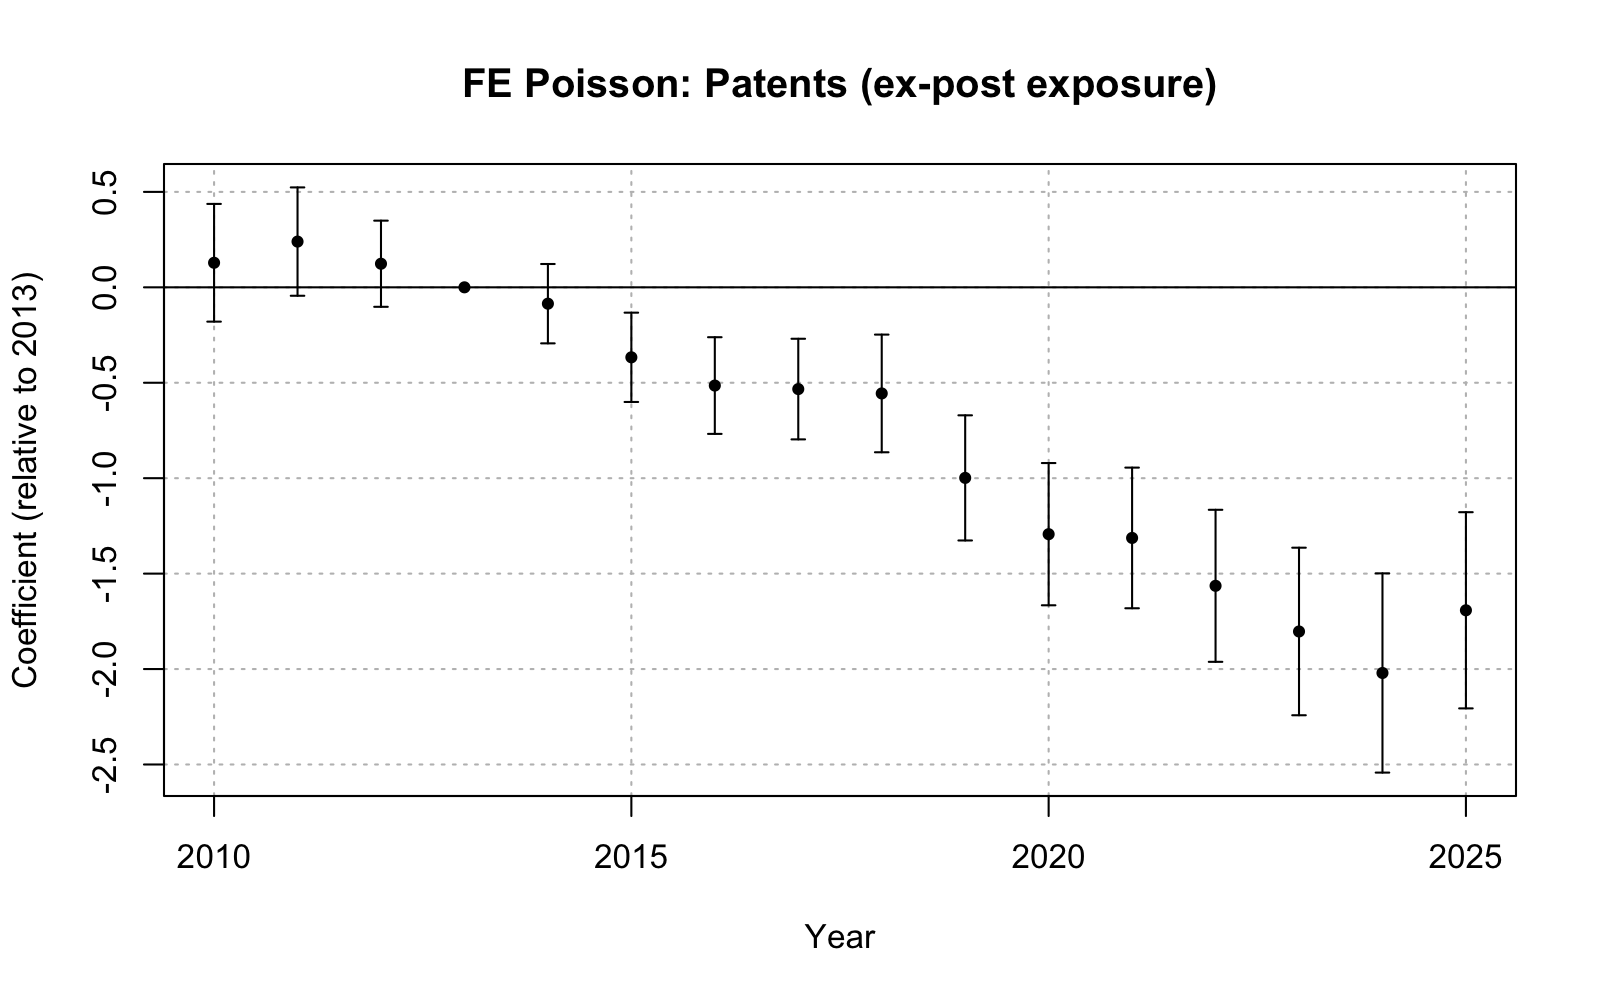
\includegraphics[width=\linewidth]{../output/RQ1/patent_poi_expost.png}
  \caption{FE Poisson event study: patents, ex-post Medicaid exposure}
  \label{fig:rob_rq1_patent_poi_expost}
\end{figure}

\begin{figure}[!h]
  \centering
  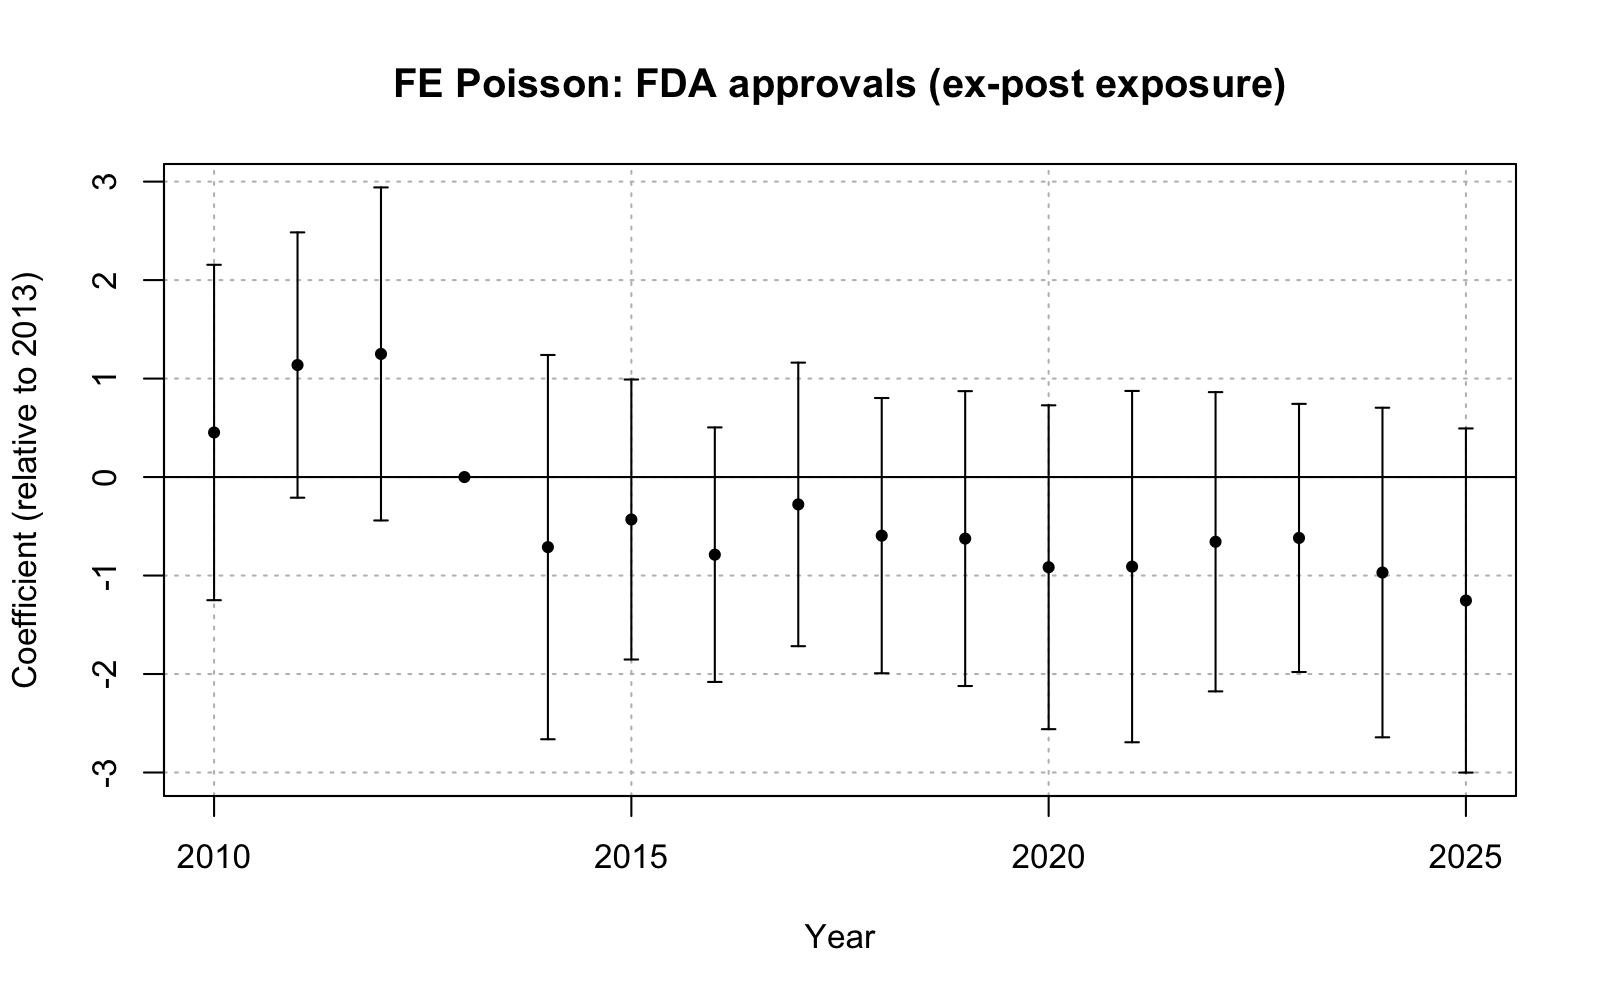
\includegraphics[width=\linewidth]{../output/RQ1/fda_poi_expost.png}
  \caption{FE Poisson event study: FDA approvals, ex-post Medicaid exposure}
  \label{fig:rob_rq1_fda_poi_expost}
\end{figure}

\clearpage

\subsection{RQ1: Binned Treatment}

\begingroup\footnotesize
\begin{table}
\centering
\begin{talltblr}[         %% tabularray outer open
entry=none,label=none,
note{}={* p \num{< 0.05}, ** p \num{< 0.01}, *** p \num{< 0.001}},
]                     %% tabularray outer close
{                     %% tabularray inner open
width=\linewidth,
colspec={Q[]X[]X[]X[]X[]},
column{2,3,4,5}={}{halign=c,},
column{1}={}{halign=l,},
hline{33}={1,2,3,4,5}{solid, black, 0.05em},
}                     %% tabularray inner close
\toprule
& \SetCell[c=2]{c} Patents && \SetCell[c=2]{c} FDA Approvals & \\
& Medium Bin & High Bin & Medium Bin & High Bin \\ \midrule
2010 & \num{-0.008}    & \num{-0.029}    & \num{0.042}   & \num{0.085}   \\
     & (\num{0.006})   & (\num{0.017})   & (\num{0.055}) & (\num{0.140}) \\
2011 & \num{-0.005}    & \num{-0.025}    & \num{0.058}   & \num{-0.064}  \\
     & (\num{0.006})   & (\num{0.016})   & (\num{0.065}) & (\num{0.105}) \\
2012 & \num{0.009}     & \num{-0.003}    & \num{0.042}   & \num{0.033}   \\
     & (\num{0.006})   & (\num{0.012})   & (\num{0.077}) & (\num{0.121}) \\
2014 & \num{0.015}**   & \num{-0.002}    & \num{0.047}   & \num{-0.091}  \\
     & (\num{0.005})   & (\num{0.011})   & (\num{0.067}) & (\num{0.130}) \\
2015 & \num{0.002}     & \num{-0.027}*   & \num{0.006}   & \num{-0.005}  \\
     & (\num{0.005})   & (\num{0.013})   & (\num{0.073}) & (\num{0.148}) \\
2016 & \num{0.007}     & \num{-0.058}*** & \num{0.158}   & \num{0.070}   \\
     & (\num{0.006})   & (\num{0.014})   & (\num{0.101}) & (\num{0.130}) \\
2017 & \num{0.005}     & \num{-0.047}**  & \num{0.239}*  & \num{0.326}   \\
     & (\num{0.006})   & (\num{0.015})   & (\num{0.114}) & (\num{0.181}) \\
2018 & \num{-0.009}    & \num{-0.075}*** & \num{0.185}*  & \num{0.213}   \\
     & (\num{0.006})   & (\num{0.017})   & (\num{0.093}) & (\num{0.155}) \\
2019 & \num{-0.004}    & \num{-0.092}*** & \num{0.071}   & \num{0.206}   \\
     & (\num{0.007})   & (\num{0.017})   & (\num{0.077}) & (\num{0.162}) \\
2020 & \num{-0.003}    & \num{-0.108}*** & \num{0.012}   & \num{0.141}   \\
     & (\num{0.006})   & (\num{0.018})   & (\num{0.092}) & (\num{0.142}) \\
2021 & \num{-0.005}    & \num{-0.118}*** & \num{0.127}   & \num{-0.048}  \\
     & (\num{0.006})   & (\num{0.018})   & (\num{0.105}) & (\num{0.182}) \\
2022 & \num{-0.010}    & \num{-0.129}*** & \num{0.101}   & \num{0.040}   \\
     & (\num{0.006})   & (\num{0.018})   & (\num{0.075}) & (\num{0.184}) \\
2023 & \num{-0.011}    & \num{-0.141}*** & \num{0.152}   & \num{0.154}   \\
     & (\num{0.006})   & (\num{0.019})   & (\num{0.087}) & (\num{0.182}) \\
2024 & \num{-0.005}    & \num{-0.142}*** & \num{0.037}   & \num{0.070}   \\
     & (\num{0.010})   & (\num{0.019})   & (\num{0.066}) & (\num{0.146}) \\
2025 & \num{-0.020}**  & \num{-0.155}*** & \num{0.010}   & \num{0.032}   \\
     & (\num{0.006})   & (\num{0.019})   & (\num{0.067}) & (\num{0.153}) \\
Num. obs. & \SetCell[c=2]{c} \num{5281696} && \SetCell[c=2]{c} \num{151200} & \\
R2        & \SetCell[c=2]{c} \num{0.534}   && \SetCell[c=2]{c} \num{0.609}  & \\
\bottomrule
\end{talltblr}
\end{table}

\endgroup

\clearpage

\subsection{RQ1: Continuous Difference-in-Differences}

\begingroup
\makeatletter
\renewenvironment{table}[1][tbp]{\@float{table}[#1]}{\end@float}
\makeatother
\footnotesize
\begin{table}
\centering
\begin{talltblr}[         %% tabularray outer open
entry=none,label=none,
note{}={* 95\% uniform confidence band does not cover 0},
]                     %% tabularray outer close
{                     %% tabularray inner open
colspec={Q[]Q[]Q[]},
column{2,3}={}{halign=c,},
column{1}={}{halign=l,},
hline{8}={1,2,3}{solid, black, 0.05em},
}                     %% tabularray inner close
\toprule
Event Time & Patents & FDA Approvals \\ \midrule %% TinyTableHeader
-3 & \num{0.0038} & \num{-0.0368} \\
   & (\num{0.0034}) & (\num{0.0602}) \\
-2 & \num{0.0023} & \num{0.0361} \\
   & (\num{0.0037}) & (\num{0.0576}) \\
-1 & \num{0.0002} & \num{-0.0326} \\
   & (\num{0.0050}) & (\num{0.0632}) \\
0 & \num{-0.0025} & \num{-0.0506} \\
   & (\num{0.0044}) & (\num{0.0731}) \\
1 & \num{-0.0126} & \num{-0.0092} \\
   & (\num{0.0055}) & (\num{0.0706}) \\
2 & \num{-0.0181}* & \num{0.0646} \\
   & (\num{0.0062}) & (\num{0.0721}) \\
3 & \num{-0.0165} & \num{0.2233} \\
   & (\num{0.0069}) & (\num{0.1018}) \\
4 & \num{-0.0189} & \num{0.1568} \\
   & (\num{0.0073}) & (\num{0.0930}) \\
5 & \num{-0.0271}* & \num{0.0861} \\
   & (\num{0.0080}) & (\num{0.0866}) \\
6 & \num{-0.0313}* & \num{0.1151} \\
   & (\num{0.0082}) & (\num{0.0846}) \\
7 & \num{-0.0315}* & \num{0.0223} \\
   & (\num{0.0084}) & (\num{0.1022}) \\
8 & \num{-0.0333}* & \num{0.0579} \\
   & (\num{0.0083}) & (\num{0.1086}) \\
9 & \num{-0.0348}* & \num{0.1329} \\
   & (\num{0.0084}) & (\num{0.1056}) \\
10 & \num{-0.0358}* & \num{0.0404} \\
   & (\num{0.0085}) & (\num{0.0921}) \\
11 & \num{-0.0324}* & \num{-0.0213} \\
   & (\num{0.0091}) & (\num{0.0919}) \\
\bottomrule
\end{talltblr}
\end{table}

\endgroup

\clearpage

\subsection{RQ2: Ex-Post FEOLS}

\begingroup\footnotesize
\begin{table}
\centering
\begin{talltblr}[         %% tabularray outer open
entry=none,label=none,
note{}={* p \num{< 0.05}, ** p \num{< 0.01}, *** p \num{< 0.001}},
]                     %% tabularray outer close
{                     %% tabularray inner open
width=\linewidth,
colspec={Q[]X[]X[]X[]X[]},
column{2,3,4,5}={}{halign=c,},
column{1}={}{halign=l,},
hline{33}={1,2,3,4,5}{solid, black, 0.05em},
}                     %% tabularray inner close
\toprule
& \SetCell[c=2]{c} Patents && \SetCell[c=2]{c} FDA Approvals & \\
& Medicaid Market Share & PDL Exposure & Medicaid Market Share & PDL Exposure \\ \midrule
2010 & \num{-0.033}    & \num{1.546}     & \num{0.285}   & \num{0.046}   \\
     & (\num{0.035})   & (\num{2.018})   & (\num{0.448}) & (\num{0.807}) \\
2011 & \num{-0.010}    & \num{0.734}     & \num{0.344}   & \num{-0.257}  \\
     & (\num{0.033})   & (\num{1.642})   & (\num{0.412}) & (\num{0.711}) \\
2012 & \num{0.005}     & \num{1.079}     & \num{0.371}   & \num{1.395}   \\
     & (\num{0.027})   & (\num{1.289})   & (\num{0.447}) & (\num{0.912}) \\
2014 & \num{-0.017}    & \num{4.161}*    & \num{-0.338}  & \num{0.398}   \\
     & (\num{0.024})   & (\num{1.890})   & (\num{0.536}) & (\num{0.647}) \\
2015 & \num{-0.088}**  & \num{0.836}     & \num{-0.037}  & \num{1.158}   \\
     & (\num{0.027})   & (\num{1.480})   & (\num{0.422}) & (\num{0.881}) \\
2016 & \num{-0.123}*** & \num{-1.554}    & \num{0.456}   & \num{2.642}   \\
     & (\num{0.032})   & (\num{1.620})   & (\num{0.418}) & (\num{1.682}) \\
2017 & \num{-0.123}*** & \num{-1.342}    & \num{1.566}*  & \num{1.924}   \\
     & (\num{0.034})   & (\num{1.890})   & (\num{0.690}) & (\num{0.992}) \\
2018 & \num{-0.136}*** & \num{-2.787}    & \num{1.181}*  & \num{1.683}   \\
     & (\num{0.037})   & (\num{1.644})   & (\num{0.563}) & (\num{1.021}) \\
2019 & \num{-0.195}*** & \num{-3.807}*   & \num{0.359}   & \num{1.171}*  \\
     & (\num{0.039})   & (\num{1.912})   & (\num{0.498}) & (\num{0.591}) \\
2020 & \num{-0.227}*** & \num{-4.650}*   & \num{0.598}   & \num{1.585}   \\
     & (\num{0.041})   & (\num{1.894})   & (\num{0.537}) & (\num{0.942}) \\
2021 & \num{-0.224}*** & \num{-5.267}**  & \num{0.103}   & \num{3.110}*  \\
     & (\num{0.040})   & (\num{1.687})   & (\num{0.583}) & (\num{1.393}) \\
2022 & \num{-0.235}*** & \num{-6.029}**  & \num{0.381}   & \num{0.994}   \\
     & (\num{0.041})   & (\num{1.941})   & (\num{0.593}) & (\num{0.653}) \\
2023 & \num{-0.240}*** & \num{-6.926}*** & \num{0.798}   & \num{1.191}   \\
     & (\num{0.041})   & (\num{1.851})   & (\num{0.583}) & (\num{1.737}) \\
2024 & \num{-0.252}*** & \num{-6.485}*** & \num{0.154}   & \num{-0.447}  \\
     & (\num{0.042})   & (\num{1.788})   & (\num{0.501}) & (\num{0.589}) \\
2025 & \num{-0.212}*** & \num{-4.589}**  & \num{-0.347}  & \num{-1.113}  \\
     & (\num{0.041})   & (\num{1.549})   & (\num{0.525}) & (\num{0.908}) \\
Num. obs. & \SetCell[c=2]{c} \num{5281696} && \SetCell[c=2]{c} \num{151200} & \\
R2        & \SetCell[c=2]{c} \num{0.535}   && \SetCell[c=2]{c} \num{0.609}  & \\
\bottomrule
\end{talltblr}
\end{table}

\endgroup

\end{document}
